\documentclass[a4paper]{article}

%\usepackage{ifpdf}
\usepackage{enumerate}


%\ifpdf % options for PDF output
 \pdfoutput=1
 \pdfcompresslevel=9
 \pdfpagewidth=8.5truein % force US letter size to match ACM template
 \pdfpageheight=11.0truein
 \usepackage[pdftex]{graphicx}
 \DeclareGraphicsExtensions{.pdf, .png, .jpg}
 \usepackage[pdftex,colorlinks=true,pdfpagemode=UseNone,pdfstartview=FitH,linkcolor=black,citecolor=black,urlcolor=blue,bookmarks=false]{hyperref}
 \usepackage[usenames]{color}%for color names
 \pdfinfo{
 /Title (PAPER TITLE)
 /Author (YOUR NAME)
 /Keywords (sensors, social network)
 }
%\else
% \usepackage[dvips]{graphicx}
% \DeclareGraphicsExtensions{.eps, .png, .jpg}
% \usepackage[usenames]{color}%for color names
% \newcommand{\url}[1]{#1} % hide hrefs
%\fi

\usepackage{url}
\usepackage{amssymb}
\usepackage[table]{xcolor}
\usepackage{pdfpages}
\usepackage{colortbl}
\usepackage{hhline}
\usepackage{pifont}
\usepackage{listings}
\usepackage{amsmath}
\usepackage{floatrow}

\newcommand\Tstrut{\rule{0pt}{2.6ex}}       % "top" strut
\newcommand\Bstrut{\rule[-0.9ex]{0pt}{0pt}} % "bottom" strut
\newcommand{\TBstrut}{\Tstrut\Bstrut} % top&bottom struts

%this is for the title page doc:
\newcommand{\HRule}{\rule{\linewidth}{0.5mm}}
% Comment this out when not in draft mode
\def\draftmode{} % useful for \ifx\draftmode\undefined<thencode>\fi in text

% $Id: macros.tex 391 2008-06-05 13:45:52Z tristan $

\usepackage{pslatex}
\usepackage{subfigure}
\usepackage[usenames]{color}
\usepackage{float}

% any local macros can go here %



%todo boxes for things.
 \ifx\draftmode\defined
  \newcommand{\todobox}[1]{}%
  \else
 \newcommand{\todobox}[1]{%
     \centering
		\fbox{\parbox[l]{\columnwidth}{\textcolor{blue}{TODO: #1}}}\\%
		%\framebox[100mm][h]{\textcolor{blue}{TODO: #1}}\\%
 }
 \fi 
 
 %reasoning boxes for things.
 \ifx\draftmode\defined
  \newcommand{\myreason}[1]{}%
  \else
 \newcommand{\myreason}[1]{%
     \centering
		\fbox{\parbox[l]{\columnwidth}{\textcolor{green}{REASONING: #1}}}\\%
		%\framebox[100mm][h]{\textcolor{blue}{TODO: #1}}\\%
 }
 \fi 
 

 %simply type \mycomment{} to get a comment box
  \ifx\draftmode\undefined
  \newcommand{\mycomment}[1]{}
  \else
 \newcommand{\mycomment}[1]{% 
            \centering
		 	\fbox{\parbox[l]{\columnwidth}{\textcolor{red}{COMMENT: #1}}}\\%
  }
  \fi 

 

% include a figure from the plots/ subdirectory
% \plot{file} will read captionm from plots/file.tex and graphic
% from plots/file.{eps,pdf}
\newcommand{\plot}[1]{%
\begin{figure}[H]
    \centerline{\resizebox{0.8\linewidth}{!}{\includegraphics{plots/#1}}}
    \caption{\label{p:#1}\protect\input{plots/#1}}
\end{figure}
}

% plot that spans both columns
\newcommand{\plotwide}[1]{%
\begin{figure*}[htbp]
    \centerline{\resizebox{0.75\linewidth}{!}{\includegraphics{plots/#1}}}
    \caption{\label{p:#1}\protect\input{plots/#1}}
\end{figure*}
}

% compare two plots
% \plot{file1,file2,caption} will show file1 and file2 side-by-side
% caption will be used for the overall caption
\newcommand{\plots}[3]{%
\begin{figure*}[tbp]
    \centering
        \label{p2:#1}
        \subfigure[{\protect\input{plots/#1}}]{
            \label{p:#1}%
            \includegraphics[width=0.34\textwidth]{plots/#1}%
        }
        \hspace{0.15\textwidth}%
        \subfigure[{\protect\input{plots/#2}}]{
            \label{p:#2}%
            \includegraphics[width=0.34\textwidth]{plots/#2}%
        }
        \caption{\protect{#3}}
\end{figure*}
}

\ifx\draftmode\undefined
% For final version
\newcommand{\comment}[1]{}%
\else
\ifpdf
% For draft mode
% ACM format doesn't like margin pars
%\newcommand{\comment}[1]{ \marginpar{$\leftarrow$}{\bf $<$#1$>$} }
\newcommand{\comment}[1]{ {\textcolor{red}{\bf $<$#1$>$}} }
\else
\newcommand{\comment}[1]{{\textcolor{red}{ \bf $<$#1$>$}}}
\fi
\fi

% Referring to a plot:
\newcommand{\plotref}[1]{Figure~\ref{p:#1}}
% or two plots:
\newcommand{\plotrefs}[2]{Figures~\ref{p:#1} and \ref{p:#2}}
% or a range of plots:
\newcommand{\plotrange}[2]{Figures~\ref{p:#1}--\ref{p:#2}}
% or a pair of plots (using \plots macro)
\newcommand{\plotsref}[1]{Figure~\ref{p2:#1}}

\newcommand{\compareplotref}[1]{Figure~\ref{p2:#1}}
\newcommand{\compareplotrefs}[2]{Figures~\ref{p2:#1} and \ref{p2:#2}}
\newcommand{\compareplotrange}[2]{Figures~\ref{p2:#1}--\ref{p2:#2}}

\title{Dissertation}
\date{\today}
\author{Martin Maciej Kukla}

%\setcounter{tocdepth}{2}
\begin{document}

%\maketitle
% title page information
\begin{titlepage} 

\begin{center}
\noindent
\huge
Learning to control double inverted pendulum with vision feedback. \\
\vspace*{\stretch{1}}
\end{center}

\begin{center}
\noindent
\huge
Martin Maciej Kukla \\
\Large
Homerton College     \\[24pt]

\includegraphics{CUni3.eps}
\end{center}

\vspace{24pt} 

\begin{center}
\noindent
\large
{\it A dissertation submitted to the University of Cambridge \\ 
in partial fulfilment of the requirements for the degree of \\ 
Master of Philosophy in Advanced Computer Science} 
\vspace*{\stretch{1}}
\end{center}

\begin{center}
\noindent
University of Cambridge \\
Computer Laboratory     \\
William Gates Building  \\
15 JJ Thomson Avenue    \\
Cambridge CB3 0FD       \\
{\sc United Kingdom}    \\
\end{center}

\begin{center}
\noindent
Email: mmk48@cam.ac.uk \\
\end{center}

\begin{center}
\noindent
\today
\end{center}

\end{titlepage} 

\newpage
\vspace*{\fill}


\newpage
{\Huge \bf Declaration}

\vspace{24pt} 

I \authorname of \authorcollege, being a candidate for the M.Phil in
Advanced Computer Science, hereby declare that this report and the
work described in it are my own work, unaided except as may be
specified below, and that the report does not contain material that
has already been used to any substantial extent for a comparable
purpose.

\vspace{24pt}
Total word count: \wordcount

\vspace{60pt}
\textbf{Signed}: 

\vspace{12pt}
\textbf{Date}:


\vfill

This dissertation is copyright \copyright 2010 \authorname. 
\\
All trademarks used in this dissertation are hereby acknowledged.



\newpage
\vspace*{\fill}


\section*{Acknowledgments}

I would like to thank my supervisor, professor Carl Rasmussen for his countless support and encouragement with the project. His insights and explanations were always enormously helpful to me. Furthermore, I am really grateful for having a possibility to work on PILCO.

\noindent I would like to thank Paavo Parmas for sharing his version of the code responsible for running the experiments. 



\begin{abstract}
what is the problem:
-control

and approach:
Probabilistic inference for control

the difficulties:
-real system

contribution in this work:
-sequence of linear models
-dynamics wrong
-dynamics extensions


\end{abstract}

\newpage


\tableofcontents
\listoffigures
%\listofalgorithms
%%%%%%%%%%%%%%%%%%%%%%%%%%%%%%%%%%%%%%%%%%%%%%%%%%%%%%%%%%%%%%%%%%%%%%%%%%%%%%%%%%%%%%%%%%%%%%%%%%%%%%%%%%%%%%%%%%%%%%%%%%%
\section{Introduction}
\label{s:intro}
The inverted pendulum is a control theory problem. The pendulum, which is freely hanging downwards, is attached to a cart\ (Figure \ref{fig:intro:initialpend}). The force can be applied to the cart, which moves it back and forth along the horizontal line. The applied force also, indirectly, moves the pendulum itself. The task is to apply the sequence of forces to a cart, which will swing the pendulum up\ (Figure \ref{fig:exps:swinguppend}) and keep it balanced in the upright position\ (Figure \ref{fig:exps:uprightpend}). In the double inverted pendulum, there is also an additional pendulum attached at the end of the first one.

\begin{figure}[!ht]
    \centering
    \begin{floatrow}
    \ffigbox[\FBwidth][\FBheight][t]{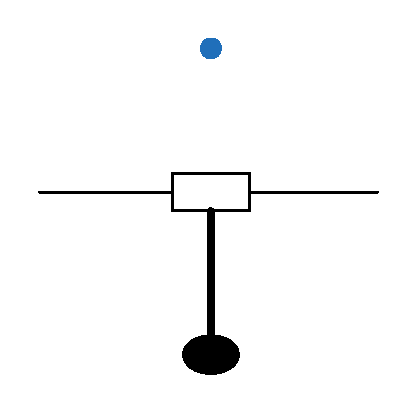
\includegraphics[width=0.3\textwidth,scale=0.4]{plots/initial_pendulum}}{\caption{The initial state: the pendulum is hanging downwards.}\label{fig:intro:initialpend}}
    \qquad
    \ffigbox[\FBwidth][\FBheight][t]{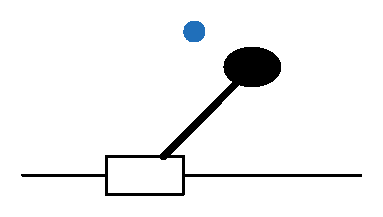
\includegraphics[width=0.3\textwidth,scale=0.4]{plots/swing_up_pendulum}}{\caption{The pendulum in the middle of the swing up action.}\label{fig:exps:swinguppend}}
    \qquad
    \ffigbox[\FBwidth][\FBheight][t]{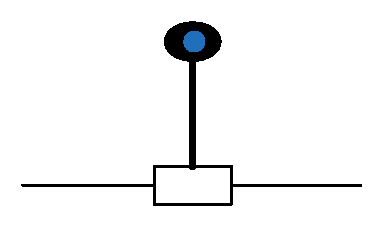
\includegraphics[width=0.3\textwidth,scale=0.4]{plots/upright_pendulum}}{\caption{The pendulum is in the upright position.}\label{fig:exps:uprightpend}}
    \end{floatrow}
\end{figure}

\noindent The task can be solved by deriving the controllers from the first principle\ (i.e., Lagrange's equations of motions). However, those controllers are task and parameters specific\ (e.g., different friction will result in a different controller). More general solution can be achieved if a controller is trained in reinforcement learning setting: an applied action is followed by a loss. The action is chosen to minimize the loss. There is only a single action in our problem, which is the force applied to a cart. The objective of the policy\ (i.e. controller) is the tip of the pendulum to be at the target: the upright position above the origin\ (the blue dot on the Figures \ref{fig:intro:initialpend}-\ref{fig:exps:uprightpend}). Thus, the loss is defined as the Euclidean distance between the tip of the pendulum and that target. 

\noindent The model-based reinforcement learning algorithm is used in this dissertation. First, the dynamics of the system is modeled solely from the data samples. The probabilistic model of the dynamics gives the predictions and its uncertainty on how the dynamical system evolves. Then, those information are used for the optimization of policy. The parameters of policy which give the predicted trajectory with the lower loss are preferable. The resulting policy is a closed-loop controller i.e. it uses information on current state for choosing next action.

\noindent The project aims to control a physical double inverted pendulum. The system is being recorded in real time using camera. The current state of the system is estimated from a frame, which introduces the noise and delay\ (the capture of frame and its transmission takes time) in observation. Basing on the estimated current state, the action is applied to the cart. Since the camera frame is a delayed version of the real state, the action itself is delayed. Finally, the velocities of the system are not directly observed from vision, which has implications to the representation of the system.

\noindent This dissertation is organized in the following order: the section \ref{s:pilco} describes the learning algorithm called \textit{PILCO}, probabilistic inference for control. It details how the dynamics and policy are being represented. It also outlines how both components are connected and trained; the section\ref{s:exps} presents the experiments with physical apparatus. It reports the results for single and double pendulum problems. The conclusions of this project can be found in the section \ref{s:con}.
\section{Probabilistic inference for control}
\label{s:pilco}
The controller is a function $\pi(x_{t})=u_{t}$, which takes a current state $x_{t}$ of the system and outputs a new action $u_{t}$ to be applied to the system. The system will then evolve according to its dynamics function $f$:
\begin{equation}
x_{t+1}=f(x_{t}, u_{t})
\end{equation}
Given the previous state $x_{t}$ and the applied action $u_{t}$, the dynamics function $f$ returns the new state of the system. Furthermore, each single state of the system $x_{t}$ has an associated cost $c(x_{t})$\ (e.g., the distance between the tip of pendulum and the upright position). For the given controller $\pi$, the total cost associated with the evolution of the system from the uncertain state i.e. $x_{1} \sim \mathcal{N}(\mu, \sigma^2)$ can be defined as $J^{\pi}$:
\begin{equation}
J^{\pi}=\sum_{t=1}^{T} \mathbb{E}[c(x_{t})]
\end{equation}
PILCO \cite{deisenroth2011pilco} is a probabilistic inference framework for learning the $\pi$ controller function which minimizes its $J^{\pi}$ total cost. 

\noindent The dynamics function of the system $f(x_{t}, u_{t})$ can be redefined as $f(\overline{x}_{t})$, where $\overline{x}_{t} \equiv [x_{t}, u_{t}]$. This nonlinear dynamics $f(\overline{x}_{t})$ can be modeled by Gaussian Processes. Different dynamics models involving Gaussian Processes are detailed in the next section \ref{s:pilco:dyn}. Given the dynamics model and the controller $\pi$, the $J^{\pi}$ total cost of the policy can be approximated by propagating uncertainty \cite{candela2003propagation} through controller and dynamics functions. 

\noindent To calculate the distribution over the next state  from the distribution over the current state: $p((x_{t}) -> p(x_{t+1})$: First, the uncertain state $x_{t} \sim \mathcal{N}(\mu, \sigma^2)$ can be propagated through the $\pi$ controller function to get a distribution over the next action: $p(u_{t})$. If the controller function is nonlinear, the output distribution is approximated as Gaussian distribution by moment matching. Next, by computing the covariance between $x_{t}$ and $u_{t}$, we construct the joint normal distribution over $x_{t}$ and $u_{t}$ defined as $p(\overline{x}_{t})$. This distribution is then propagated through the dynamics function $x_{t+1}=f(\overline{x}_{t})$. Again, since $f$ function is nonlinear, the output distribution is not Gaussian and needs to be approximated by moment matching. 

\noindent The one-step uncertainty propagation may be extended to calculate the distribution over all the states: $p(x_{1}, x_{2}, x_{3}...x_{T})$. Having the distribution over all the states, the total cost $J^{\pi}$ of the current controller can be directly computed. To learn successful controller, PILCO conditions the $\pi$ controller on its parameters $\theta$: $\pi(x_{t}|\theta)=u_{t}$. Then, the derivatives of the total cost with respect to the controller parameters $\frac{\partial J^{\pi}}{\partial \theta}$ are computed and used for optimization of $\theta$ parameters of the controller. The details of this approach can be found in Deisenroth and Rasmussen \cite{deisenroth2011pilco}.

\subsection{Dynamics model}
\label{s:pilco:dyn}

The dynamics model maps the current state $x_{t}$ and the applied action $u_{t}$ to the next state $x_{t+1}$:  $x_{t+1}=f(\overline{x}_{t})$,  where $\overline{x}_{t} \equiv [x_{t}, u_{t}]$. It is worth noticing that for the dynamics model, the applied action $u_{t}$ is treated as any other state variable. Gaussian Processes\ (GP) are chosen for modeling the dynamics, since the dynamics of inverted pendulum is nonlinear.

\noindent The single evolution of the system generates the following samples for the dynamics model: $[\overline{x}_{1}, x_{2}], [\overline{x}_{2}, x_{3}], [\overline{x}_{3}, x_{4}] [\overline{x}_{4}, x_{5}]...[\overline{x}_{T-1}, x_{T}]$, where the first position is the input to the dynamics model and the second is its output. There is a noise on inputs as well as outputs. The standard GP regression model presented in the section \ref{s:pilco:gpr} assumes the noisy outputs, but not the noisy inputs. The noise on the inputs may be ignored, so the samples can be fitted directly to the GP regression model as if the inputs were not noisy. Another approach is to filter first the noisy inputs passed to the dynamics model. The input of the sample at time $t$ is also the output of the sample at time $t-1$. The predictive distribution of the GP for the input at time $t-1$ can be used to filter the input at time $t$. This will result in the distribution on the input, which may be propagated through GP. The output distribution at time $t$ is approximated to normal distribution by moment matching. This idea is embodied in the Direct Method for Gaussian Processes Time-Series model described in the section \ref{s:pilco:ssm}.

\subsubsection{Gaussian Processes for Regression}
\label{s:pilco:gpr}
The Gaussian Processes\ (GP) model the distribution over the functions. The predictive distribution $y_*$ at any test input $x_{*}$ is Gaussian and depends on all of the training points $({\bf x}, {\bf y})$:
\begin{equation} \label{eq:gpr:preddistr}
\begin{split}
p(y_*|x_*,{\bf x},{\bf y}, \mathcal{M}_i) \sim {\cal N}\big(&{\bf k}(x_*,{\bf x})^\top [K+\sigma_{\rm noise}^2I]^{-1}{ \bf y}, \\
& k(x_*,x_*)+\sigma_{\rm noise}^2-{\bf k}(x_*,{\bf x})^\top [K+\sigma_{\rm noise}^2I]^{-1}{\bf k}(x_*,{\bf x})
\end{split}
\end{equation}
where $k(x,x')$ is a covariance function and $K$ is a covariance matrix in which $K_{ij}$ element equals to $k({\bf x}_{i}, {\bf x}_{j})$. The example of $k(x,x')$ is a squared exponential covariance function:
\begin{equation} \label{eq:gpr:covse}
k_{SE}(x,x') = v^2\exp\big(-\displaystyle\frac{(x-x')^2}{2\ell^2}\big)
\end{equation}
where the hyperparamaters are $v$-signal and $\ell$-lenghtscale\ (also, $\sigma_{\rm noise}$ in the equation \ref{eq:gpr:preddistr} is another hyperparameter).  The lengthscale $\ell$ describes how much two $x$ points should covary depending on the distance between them. If the lengthscale $\ell$ is small, the two $x$ points covary only if they are close to each other. The squared exponential is a stationary covariance function, which means that how two points covary depends only on the difference between them\ (i.e. $x-x'$), not on their absolute values. In this dissertation, the $x$ inputs are multidimensional\ (as the state of the inverted pendulum has more than one variable). We use automatic relevance determination\ (ARD) covariance function, which is a multidimensional equivalent of squared exponential covariance function while having separate $\ell$ lengthscale hyperparamaters for each dimension. 

\noindent The predictive distribution for the test input $x_{*}$ given in the equation \ref{eq:gpr:preddistr} is conditioned on $\mathcal{M}_i$, which is a linear contribution of the GP model in this dissertation. The predictive distribution for the test input $x_{*}$, which includes the linear contribution will have, additionally, its mean shifted by a linear component: $w^\top x_{*}+b$.  It is worth highlighting the fact that the GP model is a nonparametric model. The distribution over the functions is expressed directly by all of the training points.  In a sense, a single training point is a "parameter" of the model. The more training points there are available, the larger the amount of "parameters" of the GP model is.

\noindent The Figures \ref{fig:gpr:gp0}-\ref{fig:gpr:gp3} shows how the predictive distribution for all $x_{*}$ test inputs change with more training points being available. The GP with a squared exponential covariance function and the hyperparameters: lengthscale $\ell=0.5$, signal $s=1$ and the noise  $\sigma_{\rm noise}^2=0.01$, is used. This GP model does not have a linear component. The Figure \ref{fig:gpr:gp0} shows the predictive distribution for $x_{*}$ if no training points are available. The predictive distribution is the same for any test input: the mean is equal to zero and the variance is equal to $1.01$, where $s^2+\sigma_{\rm noise}^2=1.01$\ (the grey area on the diagrams corresponds to the variance being multiplied by $2$). Any new training point changes the mean and the variance of the test points in its neighborhood, where the lengthscale parameter $\ell$ defines how big the affected neighborhood is. On the Figure \ref{fig:gpr:gp3}, we can see that the GP model remains uncertain about the regions of the function, in which there were no training points. The mean and the variance for $x=-3$ is the same if there are three training points\ (Figure \ref{fig:gpr:gp3}) or no training points\ (Figure \ref{fig:gpr:gp0}).

\begin{figure}[!ht]
    \centering
    \begin{floatrow}
    \ffigbox[\FBwidth][\FBheight][t]{\includegraphics[width=60mm,scale=0.6]{plots/gp_nosamples}}{\caption{GP distribution over the functions if no training points are available.}\label{fig:gpr:gp0}}
    \ffigbox[\FBwidth][\FBheight][t]{\includegraphics[width=60mm,scale=0.6]{plots/gp_1sample}}{\caption{GP distribution over the functions if one training point is available.}\label{fig:gpr:gp1}}
    \end{floatrow}
    \begin{floatrow}
    \ffigbox[\FBwidth][\FBheight][t]{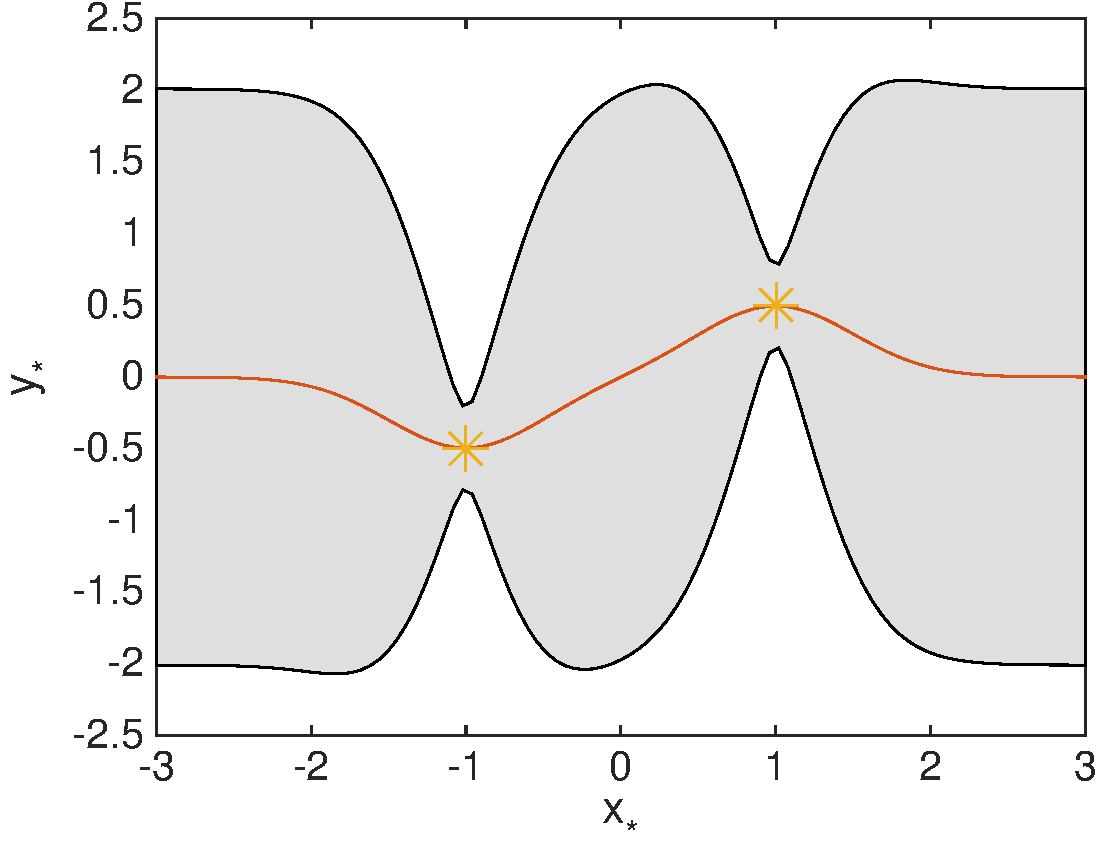
\includegraphics[width=60mm,scale=0.6]{plots/gp_2samples}}{\caption{GP distribution over the functions if two training points are available.}\label{fig:gpr:gp2}}
    \ffigbox[\FBwidth][\FBheight][t]{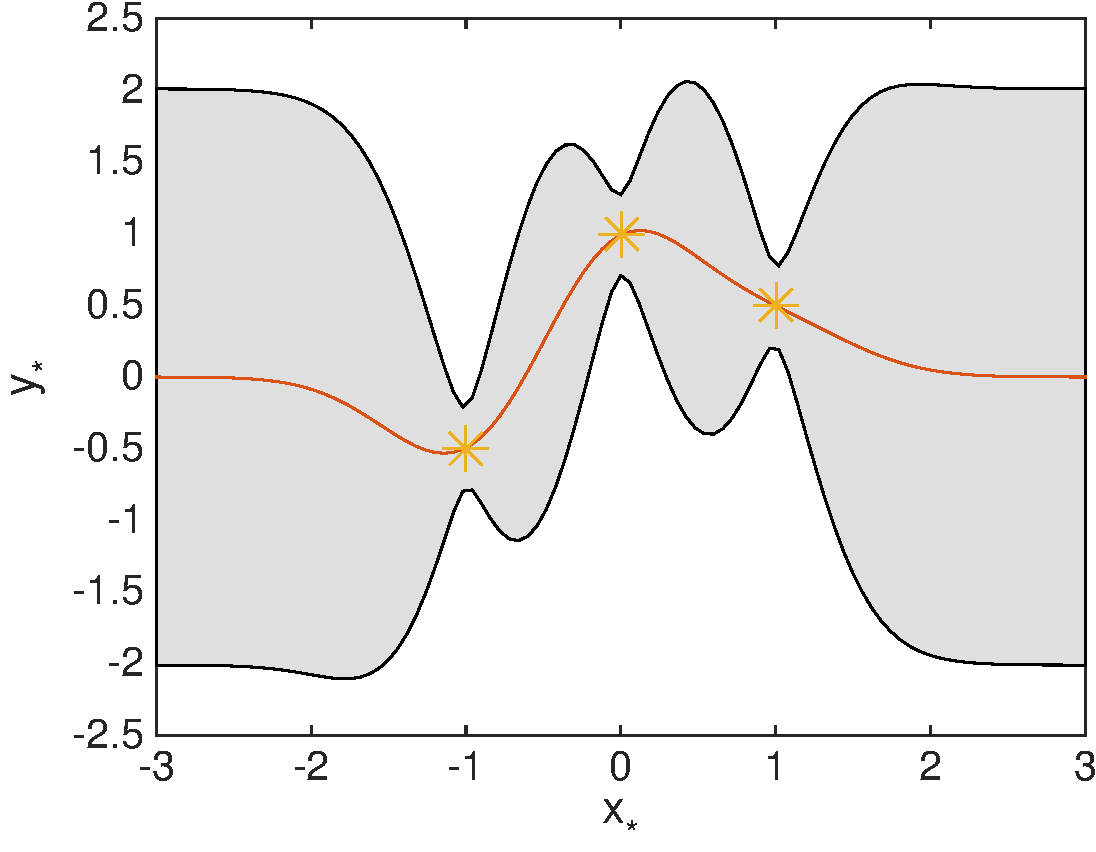
\includegraphics[width=60mm,scale=0.6]{plots/gp_3samples}}{\caption{GP distribution over the functions if three training points are available.}\label{fig:gpr:gp3}}
    \end{floatrow}
\end{figure}

\noindent The calculation of predictive distribution for the input $x_{*}$\ (equation {eq:gpr:preddistr}) involves the inversion of $[K+\sigma_{\rm noise}^2I]$ matrix. The matrix has a size of $NxN$, where $N$ is the amount of training inputs. This means that the inversion of the matrix itself has a time complexity of $\Theta(N^3)$. However, $[K+\sigma_{\rm noise}^2I]^{-1}$ can be precomputed in the training phase, since it does not depend on the test input $x_{*}$. This will result in $\Theta(N^2)$ time complexity of the prediction\ (multiplication of a matrix with a vector in variance term). Moreover, the training of the GP model involves many $\Theta(N^3)$ operations. Hyperparameters are trained by gradient based optimization of the marginal likelihood, which involves the inversion of the $K$ matrix. For hyperparamters training, this operation can't be precomputed, since $K$ matrix itself depends on the hyperparameters. More details on the inference and training in Gaussian Processes can be found in Rasmussen \cite{rasmussen2006gaussian}.

\subsubsection{Sparse Gaussian Processes}
\label{s:pilco:sgpr}

The full GP model presented in the previous section \ref{s:pilco:gpr} can be approximated by replacing the $N$ training points with $M$ pseudo points, where $M<<N$. The Figure \ref{fig:sgpr:fullgp} shows the predictive distribution of the trained GP model expressed by 9 training points, whereas the predictive distribution on the Figure \ref{fig:sgpr:sparsegp} is expressed by only using 3 pseudo points. In this toy example, we can see that both GPs model very similar predictive distribution tough they use different amount of points to express it. Second GP model used pseudo points, which are synthetic data. Pseudo points\ (i.e. pseudo inputs $\underline{x}$ and pseudo targets $\underline{f}$) are optimized to approximate the full GP. Pseudo targets $\underline{f}$ are not noisy, since $\underline{f}$ targets are not real observations, whereas the outputs $y$ of the training points for the full GP model are noisy. 

\begin{figure}[!ht]
    \centering
    \begin{floatrow}
    \ffigbox[\FBwidth][\FBheight][t]{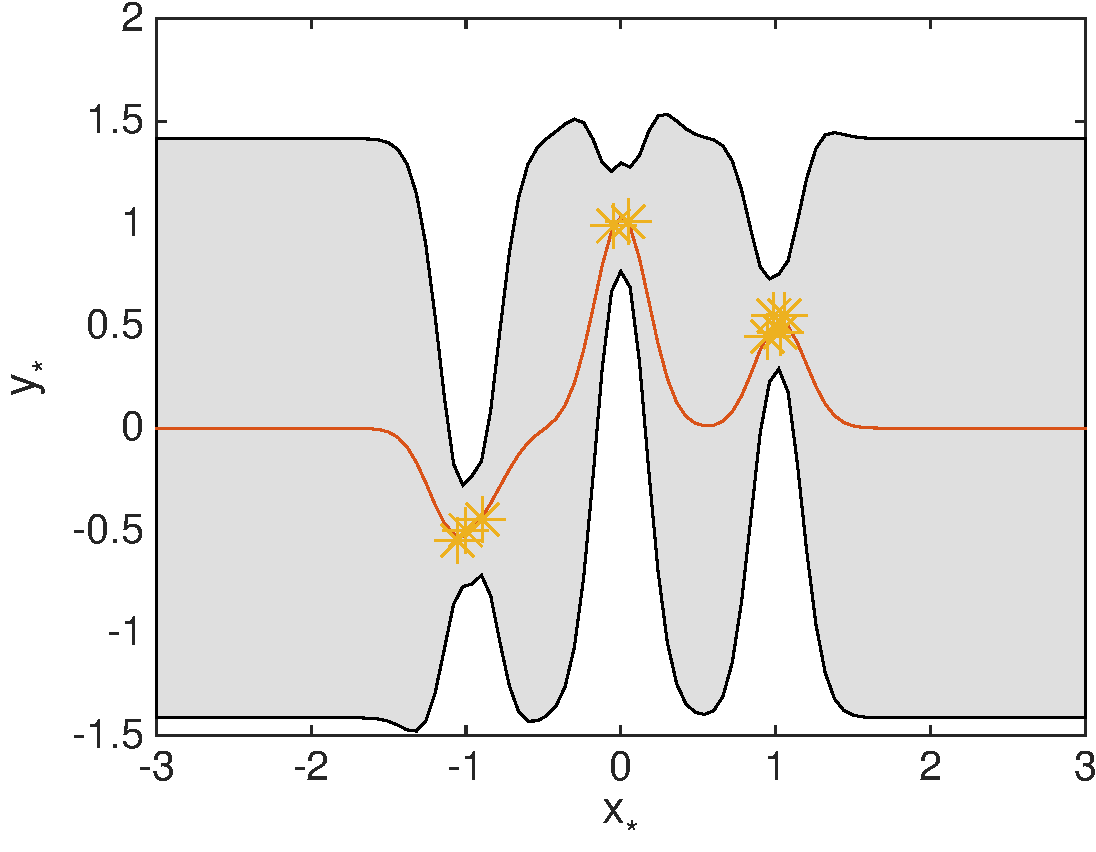
\includegraphics[width=60mm,scale=0.6]{plots/gp_full}}{\caption{The predictive distribution of the full GP model expressed by 9 training points.}\label{fig:sgpr:fullgp}}
    \ffigbox[\FBwidth][\FBheight][t]{\includegraphics[width=60mm,scale=0.6]{plots/gp_sparse}}{\caption{The similar predictive distribution of another GP model expressed by only 3 pseudo points.}\label{fig:sgpr:sparsegp}}
    \end{floatrow}
\end{figure}
 
\noindent The Fully Independent Training Conditional\ (FITC) approximation \cite{snelson2006sparse} learns the pseudo points in the following way. Assuming that the pseudo inputs $\underline{x}$ are known, it makes inference on the distribution over the pseudo targets $\underline{f}$. As the inference, we mean applying the Bayes rule to the prior on pseudo targets $\underline{f}$ and the likelihood of the training dataset $({\bf x}, {\bf y})$. Then, the posterior distribution over $\underline{f}$ can be integrated out to calculate the predictive distribution of the model for the test input $x_{*}$. To find the pseudo inputs $\underline{x}$, the gradient based optimization is applied to the marginal likelihood of the training dataset $({\bf x}, {\bf y})$. The details on the training of the FITC model can be found in Snelson and Ghahramani \cite{snelson2006sparse}. The model reduces the prediction time of the full GP from $\Theta(N^2)$ to $\Theta(M^2)$ and its training time from $\Theta(N^3)$ to $\Theta(M^2*N)$.

\noindent The FITC model can be also converted into a simpler parametric model. By taking the mean of the posterior distribution over $\underline{f}$ pseudo targets in FITC model and defining it as $\underline{\underline{f}}$, we get the parametric pseudo points: $(\underline{\underline{x}}, \underline{\underline{f}})$, where $\underline{\underline{x}} \equiv \underline{x}$. Those parametric pseudo points along with the learned hyperparameters in FITC can be directly used to model the new GP model. The prediction time of that model remains to have $\Theta(M^2)$ time complexity, but any retraining of this parametric GP model will take $\Theta(M^3)$\ (training of the Sparse GP model takes $\Theta(M^2*N)$). The Figure \ref{fig:sgpr:fullgp} shows the full GP model, whereas its parametric equivalent can be seen on the Figure \ref{fig:sgpr:sparsegp}. 

\subsubsection{Direct Method for Gaussian Processes Time-Series model}
\label{s:pilco:ssm}

To account for the noise in the inputs, the Direct Method for Gaussian Processes Time-Series model \cite{mch-thesis} can be used for modeling the dynamics. The model is shown on the Figure \ref{fig:dtsm:basic}. The latent state $x_{t}$, which is a normally distributed random variable, generates the observation $y_{t}$ while adding the Gaussian observation noise $\epsilon_{on}$ to it. Then, the latent state $x_{t}$ at time $t$ can be propagated through the parametric GP to achieve the latent state at time $t+1$, $x_{t+1}$. The Gaussian process noise, $\epsilon_{pn}$ is first added to the next latent state, $x_{t+1}$. The latent state at time $t+1$ can generate the observation $y_{t+1}$. The process may be continued till the last observation of the system $y_{T}$, which is the end of the rollout. 

\noindent The parametric GP model was presented in the previous section \ref{s:pilco:sgpr}. \underline{\underline{x}}\ and\ \underline{\underline{f}} are, respectively, the pseudo inputs and the pseudo targets of the parametric GP model. Since the parametric GP models the nonlinear function, the output distribution for propagating the Gaussian latent state $x_{t}$ as input is no longer Gaussian. That output distribution is approximated to normal distribution by moment matching. Consequently, each of the latent states $x_{t}$ is normally distributed.

\begin{figure}[H]
\centering
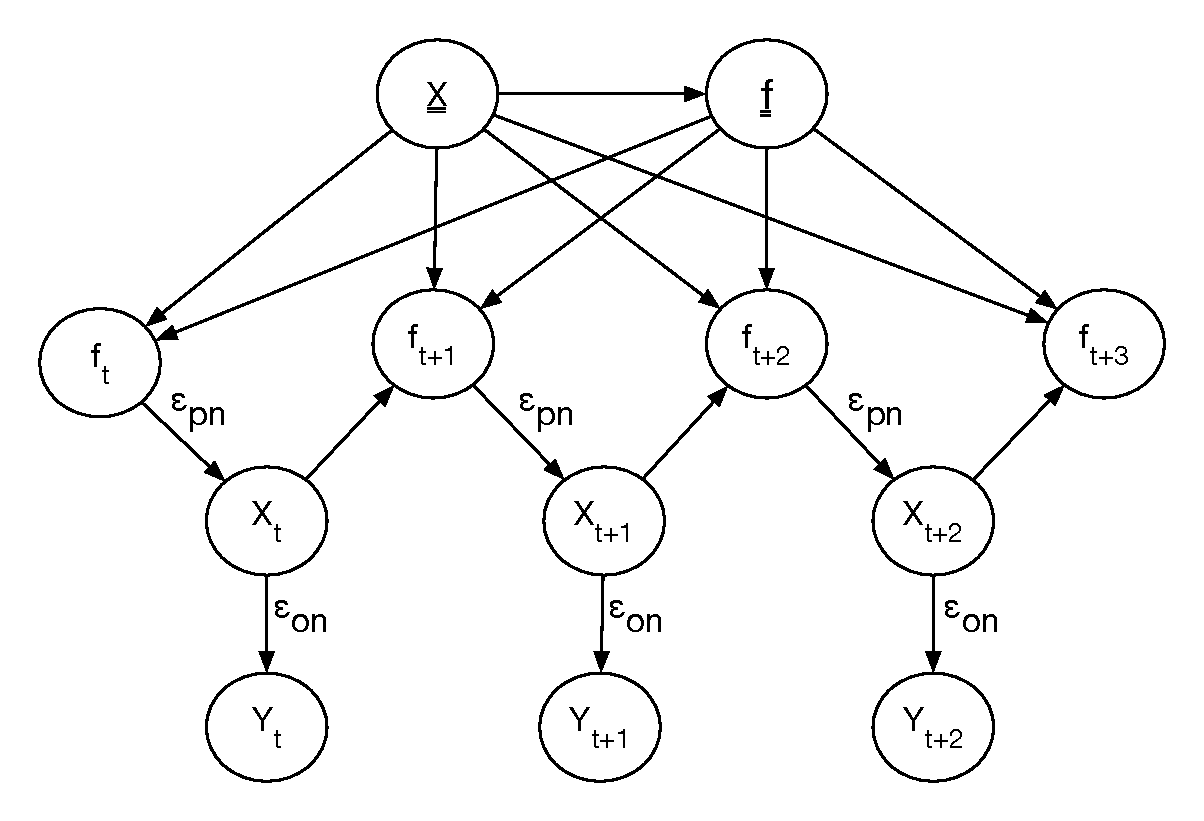
\includegraphics[width=1\textwidth, scale=1]{plots/ssm_model}
\caption{\label{fig:dtsm:basic}The Direct Method for Gaussian Processes Time-Series model in which: $y_{t}$ is a noisy observation of the state at time $t$; $x_{t}$ is a distribution over the latent state at time $t$; \underline{\underline{x}}\ and\ \underline{\underline{f}}\ are the pseudo inputs and the pseudo targets of the parametric GP model; $\epsilon_{pn}$ and $\epsilon_{on}$ stand for process and observation noise respectively.}
\end{figure}

\noindent There are the three levels of noise in the model: observation noise $\epsilon_{on}$, process noise $\epsilon_{pn}$ and the noise hyperparameter of the parametric GP $\sigma_{\rm noise}$. Only observation noise $\epsilon_{on}$ is not being propagated to the next latent state $x_{t+1}$. Process noise $\epsilon_{pn}$ and the noise of the parametric GP $\sigma_{\rm noise}$ are being added to all of the latent states $x_{1:T}$.

\noindent We can also write the marginal likelihood of the observations under the Direct Method for Gaussian Processes Time-Series. We define: $\theta := [\underline{\underline{x}}, \underline{\underline{f}}, \epsilon_{pn}, \epsilon_{on}, GP_{hyp}]$, where $GP_{hyp}$ stands for the hyperparameters of the parametric GP model. Then, the likelihood for the model can be written in the following way:
	
\begin{equation} \label{eq:ssm:lik}
\begin{split}
p(y_{1:T}|\theta) & = p(y_{1:T}|x_{1:T},\theta) p(x_{1:T}|\theta) \\
& =	p(y_{1:T}|x_{1:T},\theta) p(x_{1}| \theta) \prod_{t=2}^{T} p(x_{t}|x_{t-1}, \theta)
\end{split}
\end{equation}

\noindent The latent state at time $t$ depends only on the previous latent state at time $t-1$, not on any of the earlier latent states $x_{1:t-2}$. This Markovian property makes the Direct Method for Gaussian Processes Time-Series model tractable. The parameters $\theta$ are trained by gradient based optimization of the marginal likelihood \ref{eq:ssm:lik}. A single propagation of uncertain input through a parametric GP with precomputed inverse of covariance matrix has a time complexity of $\Theta(M^2)$, where $M$ is the amount of pseudo points. The derivative of the mean and variance of the output distribution with respect to the hyperparamaters and the pseudo targets of the parametric GP model can be also calculated in $\Theta(M^2)$ time. This uncertain input propagation needs to be conducted ${T}$ for each rollout (i.e. $[x_{1},x_{2}, x_{3},...x_{T}$). Therefore, the total time complexity of the single training iteration will be $\Theta(R*T*M^2)$, where $R$ is the amount of the rollouts. However, the operation can be made in parallel, since the computation of the prediction and derivatives for each of the rollouts are independent\ (the respective derivatives only need to be added at the end). More details on the Direct Method for Gaussian Processes Time-Series model can be found in McHutchon, Chapter 3 \cite{mch-thesis}.

\noindent In the above Direct Method for Gaussian Processes Time-Series model, only the hyperparameters and the pseudo targets are trained. The pseudo inputs may be pre-trained in the GP model which assumes noise-free inputs\ (e.g., full GP or sparse GP converted to the parametric GP). In this dissertation, the Direct Method for Gaussian Processes Time-Series model was extended to also optimize the pseudo inputs. The computation of the derivatives of the parametric GP's output distribution $x_{t+1}$ for an uncertain input $x_{t}$ with respect to the pseudo inputs has a time complexity of $\Theta(M^3)$. This makes the single iteration of the training procedure to have the time complexity of $\Theta(R*T*M^3)$. 

\begin{figure}[H]
\centering
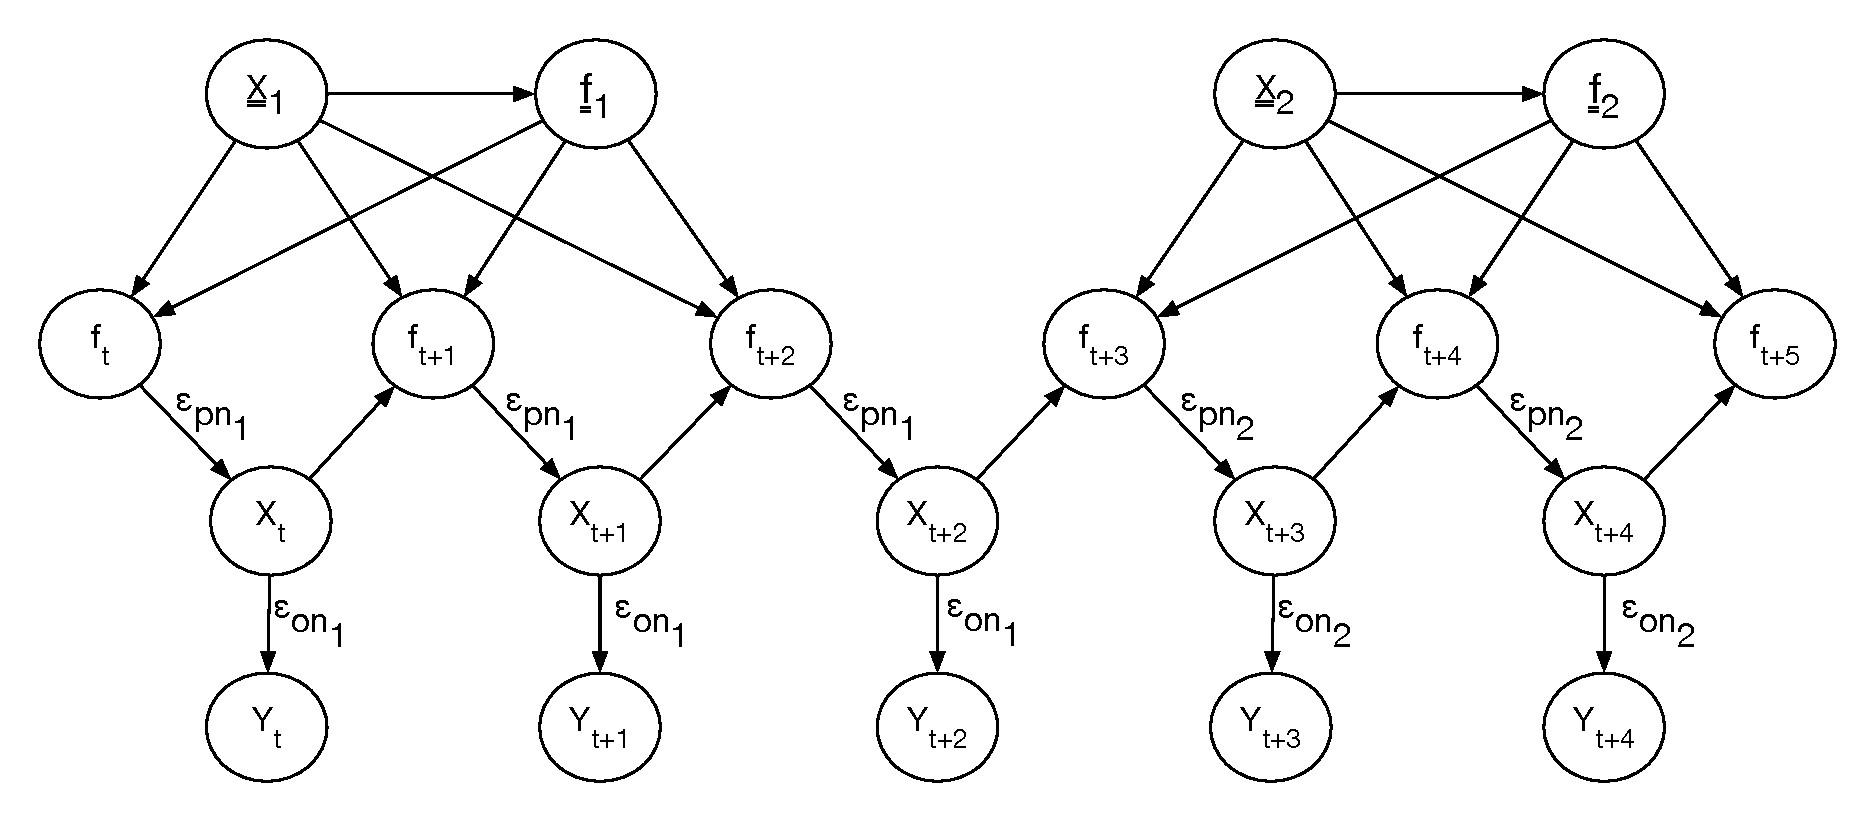
\includegraphics[width=1\textwidth, scale=1]{plots/ssm_models}
\caption{\label{fig:dtsm:twogps}The Direct Method for Gaussian Processes Time-Series model with two parametric GP models.}
\end{figure}

\noindent The Direct Method for Gaussian Processes Time-Series model may also use more than one parametric GP. The Figure \ref{fig:dtsm:twogps} shows the model in which two parametric GPs are used\ (there are two sets of pseudo points $\underline{\underline{x}}_1, \underline{\underline{f}}_1$ and $\underline{\underline{x}}_2, \underline{\underline{f}}_2$). In this model, there are also two separate sets of noise levels\ (process noises: $\epsilon_{pn_{1}}$ and $\epsilon_{pn_{2}}$, observation noises: $\epsilon_{on_{1}}$ and $\epsilon_{on_{2}}$). Although twice as many pseudo inputs are used, the output distribution for the uncertain input is calculated as many times as if the single parametric GP model was used. The time complexity of one training iteration remains to be $\Theta(R*T*M^3)$. However, there are twice as many parameters to optimize, which influences the amount of training iteration needed to find the sufficient approximation of the Hessian matrix in the BFGS algorithm used in this dissertation.

\noindent In the new model, the different dynamics models\ (i.e. parametric GPs) are used depending on which time step the rollout is at. This assumption seems unreal, since the physics of motion of the inverted pendulum does not change depending on time. However, time $t$ itself may be strongly correlated with the latent state $x_{t}$ e.g., at time $t_{k}$ the pendulum is usually having a high, positive angular velocity. By using different dynamics depending on time $t$, we effectively split the domain of the latent state $x_{t}$ into the few subdomains and use separate dynamics model for each of them. The switching between the different parametric GP models could also happen directly basing on the current latent state $x_{t}$. Those issues are further discussed, when the model is applied to the double inverted pendulum problem in the section \ref{s:exps:double:dyns}.

\noindent The Direct Method for Gaussian Processes Time-Series model requires to specify the amount of the pseudo points $(\underline{\underline{x}}, \underline{\underline{f}})$ being used. As mentioned earlier, the pseudo inputs\ \underline{\underline{x}}\ are pre-trained using the Sparse GP model. We compare the marginal likelihood of the observed data under the Sparse GP and the full GP models to determine how many pseudo points to use. If the marginal likelihood under the Sparse GP model is worse, more pseudo points should be added to the Gaussian Processes Time-Series model.

\subsection{Policy model}
\label{s:pilco:pol}
The closed-loop controller $\pi$ chooses the action $u$ to be applied depending on the current state of the system: $\pi(x_{t})=u_{t}$. As described earlier, to evaluate the policy, the uncertain state $p(x_{t})$ is propagated through the controller. This gives the distribution over the action $p(u_{t})$. The controller also keeps track on how the variables of the state $x_{t}$ covary with the action $u_{t}$. This way, the predictive variance on the future state of the system is being controlled. The Figure \ref{fig:pol:variancext} shows the linear relationship between the uncertain current state $x_{t}$ and the action $u_{t}$. The applied action results in the reduced variance on state $x_{t+1}$ on the Figure \ref{fig:pol:variancext1}. The variance is also being added to the system, since the controller performs a specific task like swinging up the pendulum.

\begin{figure}
    \centering
    \begin{floatrow}
    \ffigbox[\FBwidth][\FBheight][t]{\includegraphics[width=60mm,height=40mm]{plots/variance_state_t}}{\caption{The uncertain state $x_{t}$ with standard deviation equalled to $0.5$. There is a linear relationship between the state  $x_{t}$ and the applied action $u_{t}$ chosen by the closed-loop controller.}\label{fig:pol:variancext}}
    \ffigbox[\FBwidth][\FBheight][t]{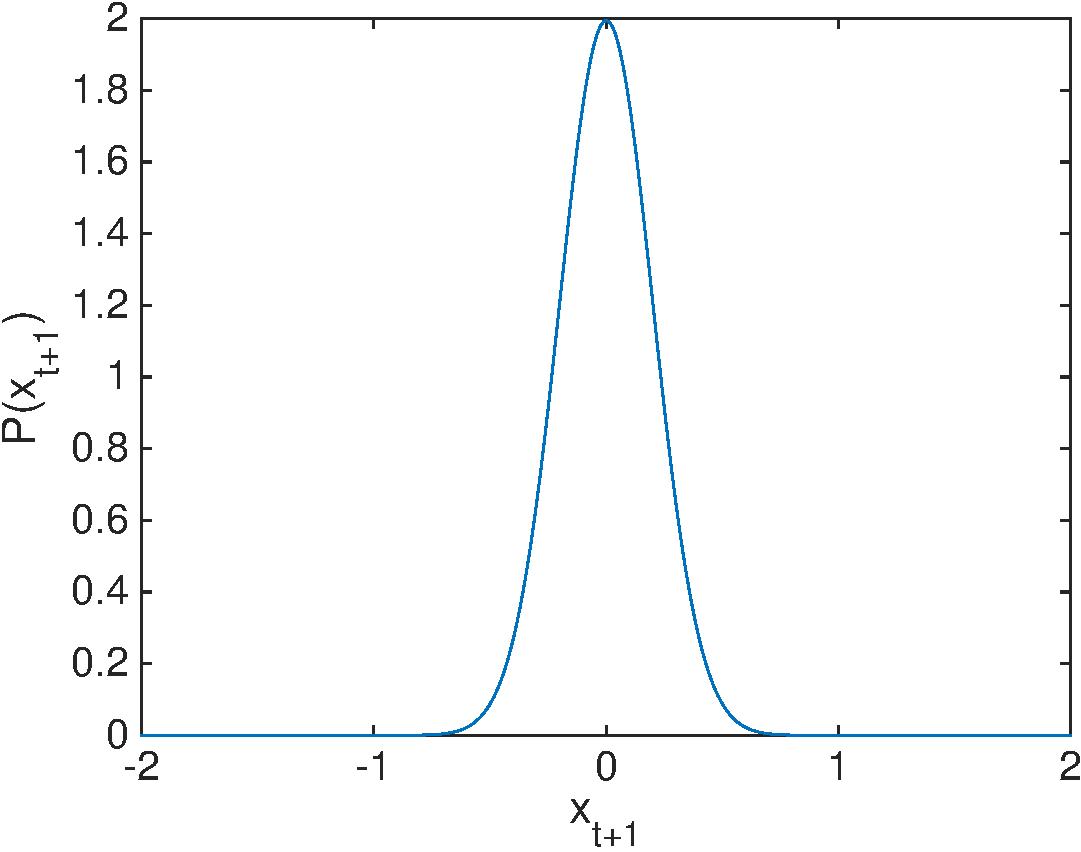
\includegraphics[width=60mm,height=40mm]{plots/variance_state_t_1}}{\caption{The uncertain state $x_{t+1}$ with standard deviation equalled to $0.2$}\label{fig:pol:variancext1}}
    \end{floatrow}
\end{figure}

\noindent The range of actions which can be applied to the real system is limited. The inverted pendulum physical apparatus used in this dissertation allows to pass the force values between $-10$ and $10$. That's why the unlimited policy output $u$ is saturated through the squashing function $sat(u)$. This operation gives action $\overline{u}$ in the requested range:
\begin{equation}
\overline{u} = sat(u) = 10 * \frac{9 * sin(u) + sin (3 * u)}{8}
\end{equation}

\subsubsection{Radial Basis Function network}
\label{s:pilco:rbf}
The radial basis function\ (RBF) network models the nonlinear function as the sum of radial basis function units:
\begin{equation}
\varphi(x) = \sum_{i=1}^{N} y_{i} exp (\frac{-(x-x_{i})^2}{2 \ell^2})
\end{equation}
where $x_{i}$ are the centers of the Gaussian bumps, $y_{i}$ are their heights and $\ell$ is a shared width. The amount of the parameters for the RBF network equals to $2*N$.

\subsubsection{Sequence of Linear models}
\label{s:pilco:seqlin}
Although the RBF network can model the nonlinear function, only its linear approximations are involved in the training. While optimizing the policy, PILCO approximates the output distribution over $u_{t}$ from $\pi$ controller by moment matching. The distribution over $u_{t}$ is Gaussian and can be achieved from $u_{t}$ directly by using linear model instead of linear approximation of the nonlinear RBF network. The parameters of the RBF network are optimized, so the trajectory after applying forces $p(u_{1}), p(u_{2}), p(u_{3})...p(u_{T})$ will be the most cost effective. Each of the action distributions $u_{t}$ can be achieved by a linear model $\pi_{t}(x)$.  Effectively, the RBF network can be replaced by $T$ linear models: $(\pi_{1}(x), \pi_{2}(x), \pi_{3}(x)),...\pi_{t}(x))$. The sequence of linear models was designed and used in this dissertation.

\noindent The amount of parameters in the sequence of linear models for one dimensional problem will be $2*T$\ (bias plus one weight per one linear model). In most scenarios, this amount of the parameters will be similar to the RBF network. The sequence of the linear models makes the controller time dependent i.e. for the same $x$ state, different actions $u_{t}$ will be chosen depending on the time $t$. The parameters of the sequence of linear models are less coupled, since there is no time interference between the linear models $\pi_{i}$ and $\pi_{j}$. The RBF network by changing its parameters to improve the policy at time $t$ will also affect the policy at time $t+1$, since the states $x_{t}$ and $x_{t+1}$ are likely to be similar. This is further discussed in the section \ref{s:exps:double:policyrep}.

\subsection{PILCO training}
\label{s:pilco:training}
First, we conduct the initial rollout in which random actions $u_{t}$ are applied. This yields the dataset: $[\overline{x}_{1}, x_{2}], [\overline{x}_{2}, x_{3}],...[\overline{x}_{T-1}, x_{T}]$, which is solely used for training the dynamics model. Then, by using the trained dynamics model, the policy model can be trained to arrive at the new $\pi$ controller. This controller is used for selecting actions $u_{t}$ in the new rollout. The dynamics and policy models training can be then repeated. For the dynamics training, all of the rollouts will be always used. The PILCO training iteration may be repeated as many times it is needed to successfully learn the control task. In training iteration, the policy model is retrained, instead of being trained from scratch. This means that the initial parameters of the $\pi_{r}$ controller are equal to the trained parameters of the $\pi_{r-1}$ controller, where $\pi_{r}$ stands for the controller after the rollout $r$.
\section{Experiments with physical apparatus}
\label{s:exps}
The experiments with the inverted pendulum are run on the physical apparatus. The Figure \ref{fig:exps:componentsrollout} shows the components involved in making the new rollout. The new frame depicting the physical pendulum arrives at the local PC every $33$ ms. The state of the pendulum is then extracted from the frame. Basing on the state, the controller chooses the action to be applied. These two operations made by the local PC take negligible amount of time. Next, the action chosen by the controller is applied to the physical apparatus. The real state at time $t$ is used to apply the action at time $t+\Delta t$. The time delay $\Delta t$ is a result of capturing the state of the pendulum on the frame by the camera, sending the frame over to the computer and applying the new action. Before the new action $u_{t}$ is applied to the pendulum, the old action $u_{t-1}$ keeps being applied.

\begin{figure}[H]
\centering
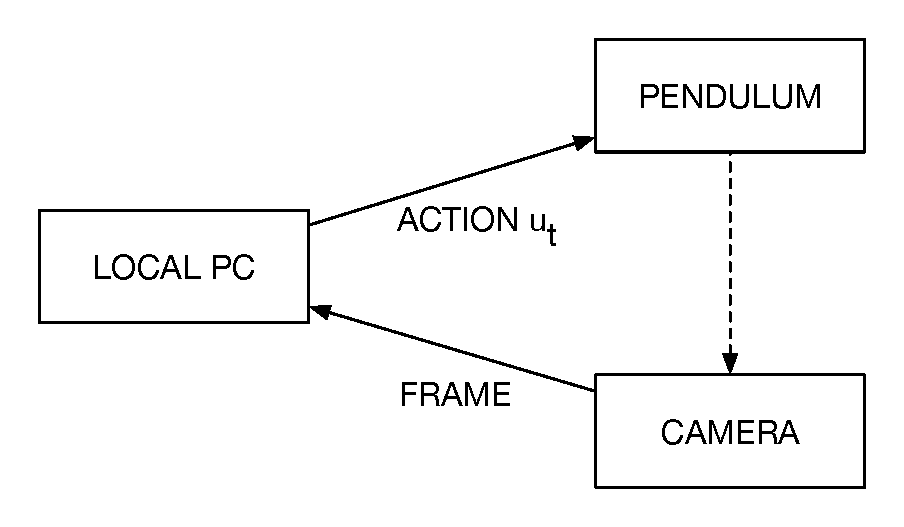
\includegraphics[width=0.5\textwidth, scale=0.5]{plots/rollout_components}
\caption{\label{fig:exps:componentsrollout} The components involved in the rollout of the physical pendulum. }
\end{figure}

\noindent Playstation 3 Eye is a cheap web camera used in this dissertation. It captures $30$ frames per second with the spatial resolution of $640x480$. Ignoring aberration effects, the move of the cart by one pixel in frame corresponds to $2$ mm distance move in the scenery. The Figures \ref{fig:exps:frame_single} and \ref{fig:exps:frame_double} show the example frames for single and double pendulum. The coloured blobs are attached to the cart and the ends of the pendulums. A color tracking algorithm is used to detect those points: a frame is converted into HSV\ (hue-saturation-value) color space and the pixels are masked, so only the pixels of the specific color\ (i.e. orange) are left. Then, the first moment of the locations of those pixels is calculated. Effectively, we calculate the center of the coloured blob. Indeed, the first moments marked as crosses, are at the centers of the coloured blobs on the Figures \ref{fig:exps:frame_single} and \ref{fig:exps:frame_double}. It is worth mentioning that the used color tracking algorithm is not lighting invariant (e.g., sunshine through the windows would affect its results).

\begin{figure}[!ht]
    \centering
    \begin{floatrow}
    \ffigbox[\FBwidth][\FBheight][t]{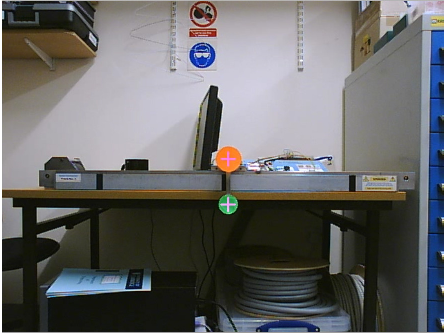
\includegraphics[width=60mm,scale=1]{plots/frame_single}}{\caption{The example frame with the single pendulum.}\label{fig:exps:frame_single}}
    \ffigbox[\FBwidth][\FBheight][t]{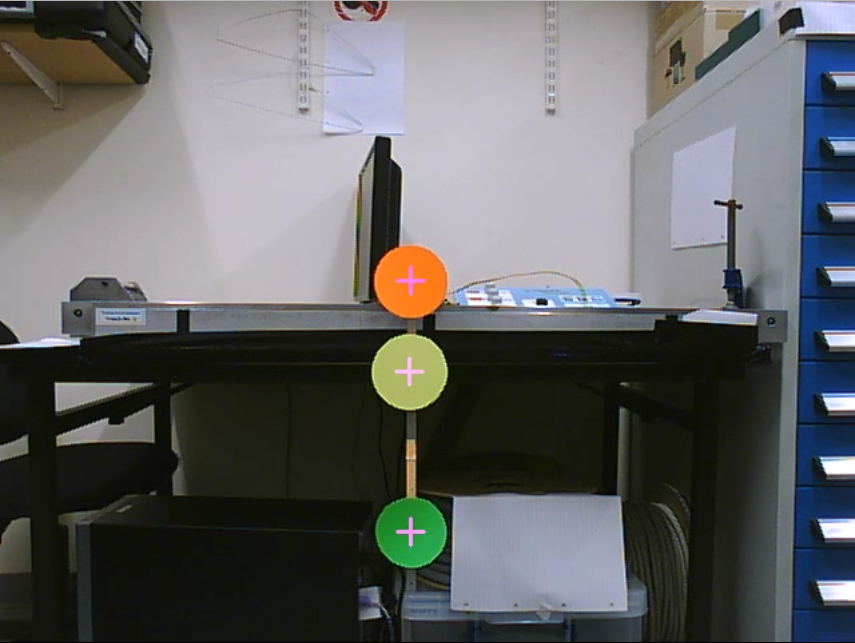
\includegraphics[width=60mm,scale=1]{plots/frame_double}}{\caption{The example frame with the double pendulum.}\label{fig:exps:frame_double}}
    \end{floatrow}
\end{figure}

\noindent For the running time speed, the program for making the rollouts is written in C/C++. It uses OpenCV library for communicating with the camera. The rollout data is sent from the local PC to the remote PC, which has 6 CPU cores. Next, the remote PC runs the PILCO framework written in MATLAB to learn the dynamics and policy models. Finally, the trained controller is sent back to the local PC and can be used for making the consecutive rollout.

\subsection{State representation}
\label{s:exps:state}
The color tracking algorithm presented in the previous section returns the current position of the cart $x$, as well as the ends of the pendulums. Those coordinates can be used to calculate the angles of the pendulums i.e. $\theta$ for the single pendulum problem. The full representation of the dynamical system also requires the cart velocity and the angular velocities of the pendulums. The velocities can be directly approximated from the previous and current values of $x$ and $\theta_{1}$. We know that the time difference between two consecutive frames is $dt=33ms$. The cart velocity can be approximated as $\dot{x}=\frac{x-ox}{dt}$, where $ox$ stands for the cart position from the previous frame. The full state representation for the single pendulum problem would be then:
\begin{equation}
[ou, x, \theta, \dot{x}, \dot{\theta}, u] \nonumber
\end{equation}
where $ou$ is the previous action applied to the system. As explained earlier, the action $u$ is applied with the time delay, and thus, the previous action $ou$ is also needed for the full representation of the state. 

\begin{figure}[H]
\centering
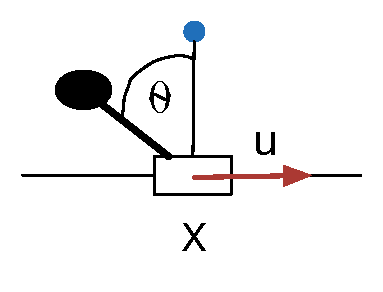
\includegraphics[width=0.5\textwidth, scale=0.5]{plots/pendulum_maths}
\caption{\label{fig:exps:statepend} The pendulum with the marked variables of the state.}
\end{figure}

\noindent The dynamics model for the above representation needs to predict 4 variables: $[x, \theta, \dot{x}, \dot{\theta}, u]$. Effectively, in PILCO, there will be a separate GP model for each variable. Each model will have its own noise level for the predicted variable. However, we know that there are only two noise sources per frame: noises on current cart position and the current end of the pendulum. PILCO would assume more noise sources than there, actually, are in the system.

\noindent The full state of the dynamical system can be also described by second order Markov representation. Instead of
approximating velocities, we can pass the previous and current $x$ and $\theta$ variables directly to the dynamics model. The belief is that the GP model itself will learn how to model the velocities out of those variables. Effectively, the state representation for the single pendulum would be then:
\begin{equation}
[oou, ox, o\theta, ou, x, \theta, u] \nonumber
\end{equation}
where $oou$ stands for the action applied before the previous frame; $ox$ and $o \theta$ are, respectively, a cart position and a pendulum angle extracted from the previous frame. 

\noindent The dynamics model for the second order Markov representation will try to predict only two variables: $x$ and $\theta$, since the rest of the new state representation can be copied over from the previous state. In PILCO, the dynamics model will consist of two GP models. This means that the dynamics will assume two sources of noise, which matches the amount of noise levels in the real system. Fewer GP models also shortens the training time of the PILCO framework.

\subsection{Delay and noise levels}
\label{s:exps:delaynoise}
The dynamics model does not need to know what the time delay is in the system. It can abstract over this parameter as long as the state of the dynamical system is fully represented. Full representation means that having the current state of the system, the next state of the system can be calculated in deterministic way. It is worth thinking how the full representation of the system would depend on different time delays. Frames from the camera come at the constant interval of $33$ ms and the delayed actions are believed to be also applied at the same constant interval. On the Figure\ref{fig:exps:camdelay}, the frames and the delayed actions are represented as $f_{t}$ and $a_{t}$, respectively, on the time axis. In this pictorial scenario, to calculate the frame $f_{t+1}$, we need two previous frames\ (i.e. second order Markov representation) along with all the actions, which affect those frames\ (including the calculated frame $f_{t+1}$). This mean that for calculating $f_{t+1}$, we need the following input: $[a_{t-2}, f_{t-1}, a_{t-1}, f_{t}, a_{t}]$. This is equivalent to the full representation of the inverted pendulum presented in the previous section. 

\begin{figure}[H]
\centering
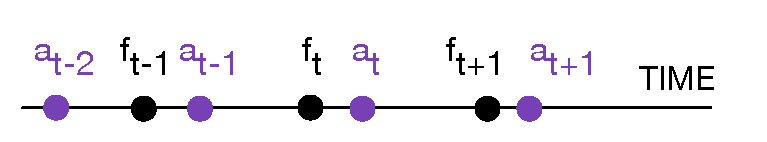
\includegraphics[width=0.5\textwidth, scale=0.5]{plots/cam_delay}
\caption{\label{fig:exps:camdelay} The frame $f_{t}$ and the delayed actions $a_{t}$ on the time axis. It presents the situation when the time delay is lower than the time between frames i.e. $33$ ms.}
\end{figure}

\noindent The time delay on the Figure \ref{fig:exps:camdelay} is represented as the time difference between applying the action $a_{t}$ and the frame $f_{t}$ itself. The higher time delay would mean that $a_{t}$ points are shifted in right direction. If the time delay is higher that the time difference between two consecutive frames, the $f_{t-1}$ frame would be affected by the action $a_{t-3}$. This changes the full representation of the system by adding older action $a_{t-3}$ to it. Thus, to determine whether the time delay in our experiments was higher than $33$ ms, the third order Markov representation\ (i.e. including action $a_{t-3}$) dynamics model was used. The linear component of the trained dynamics model had a very low value on the oldest action $a_{t-3}$. This was treated as an indicator that the dynamics can be successfully model without the additional action added. This effectively means, that the time delay is less than $33$ ms.

\noindent The locations of the coloured pixels are averaged to calculate the position of interests e.g., the cart position. The blobs themselves are the circles whose diameters equal to $20$ pixels. Each of those pixels represent the line along which the locations are averaged to get a horizontal position $x$ of the center of the coloured blob. Effectively, we have $20$ estimations of $x$ positions. For double inverted pendulum, the blobs were increased to the diameters of $49$ pixels to further reduce the noise level.

\subsection{Single pendulum}
\label{s:exps:single}
The experiments with the single physical pendulum of $12.5$ cm length were conducted. As mentioned earlier, the state of the system is described by the second order Markov representation:
\begin{equation}
[oou, ox, o \theta, ou, x, \theta, u] \nonumber
\end{equation}
There are $6$ state variables, where two of them\ (i.e. $x, \theta$) needs to be predicted by the dynamics model. As a policy model, the RBF network with $50$ radial basis functions is used. For PILCO dynamics model, there are $50$ pseudo points being used. For training the dynamics model as well as policy, $300$ iterations of BFGS algorithm is applied after each rollout. A single rollout lasts almost $2$ seconds, which corresponds to $60$ new samples for the dynamics model\ ($T=60$). The rollout can stop earlier if the cart hits one of the sides of the physical apparatus i.e. fail-safe mechanism\ (the pendulum track has the length of around $80$ cm: there is $40$ cm from the center to hit the side).

\noindent The trained dynamics model for this representation switched off the nonlinear GP model for cart position $x$by setting one of its length scale hyperparameters to very low value\ (i.e. $0.01$). At the same time, the linear part of the dynamics model behaves as expected: it models the next $x^{*}$ cart position by using previous and current cart positions, $ox$ and $x$:
\begin{equation}
x^{*} = 1.79 \times x - 0.79 \times ox = x + 0.79 \times (x-ox) \nonumber
\end{equation}
The next $x^{*}$ cart position is a current cart position plus its velocity. However, during the joint optimization of the linear and nonlinear model, this linear model is not known to the nonlinear GP model. At that time, the nonlinear GP thinks that it can not explain the data at all, and thus, it decides to switch itself off by setting very low length scale. The optimization procedure does not manage to switch the nonlinear GP on once the good linear model is achieved. This problem is mitigated if the linear components of the dynamics model are initialized more reasonable i.e. $2$ is a weight for $x$ and $-1$ for $ox$. Also, after rollout nr $13$, when there are $602$ training points for nonlinear GP, the $50$ pseudo points is not enough for modeling the dynamics. This is diagnosed by comparing the marginal likelihood of the full GP with sparse GP model as it was mentioned in the section \ref{s:pilco:ssm}. The amount of pseudo points is increased to $100$ from that rollout onward.

\noindent After $20$ rollouts and the total exposure of around $36$ seconds\ (i.e. $1074$ dynamics samples), the successful controller is learned by PILCO. Again, the dynamics's linear weights model the velocities:
\begin{equation}
\begin{split}
x^{*} = 1.76 \times x - 0.76 \times ox = x + 0.76 \times (x-ox) = x + 0.76 \times \dot{x} \\ \nonumber
\theta^{*} = 1.95 \times \theta - 0.95 \times o \theta = \theta + 0.95 \times (\theta-o \theta) = \theta + 0.95 \times  \dot{\theta} \nonumber
\end{split}
\end{equation}
The noise levels of the dynamics model are low. There is a $0.2^{\circ}$ observation noise on $\theta$. However, the observation noise is not propagated through the time-series model. All of the noise levels on $x$ are less than $0.025$ cm. 

\begin{figure}[!ht]
    \centering
    \begin{floatrow}
    \ffigbox[\FBwidth][\FBheight][t]{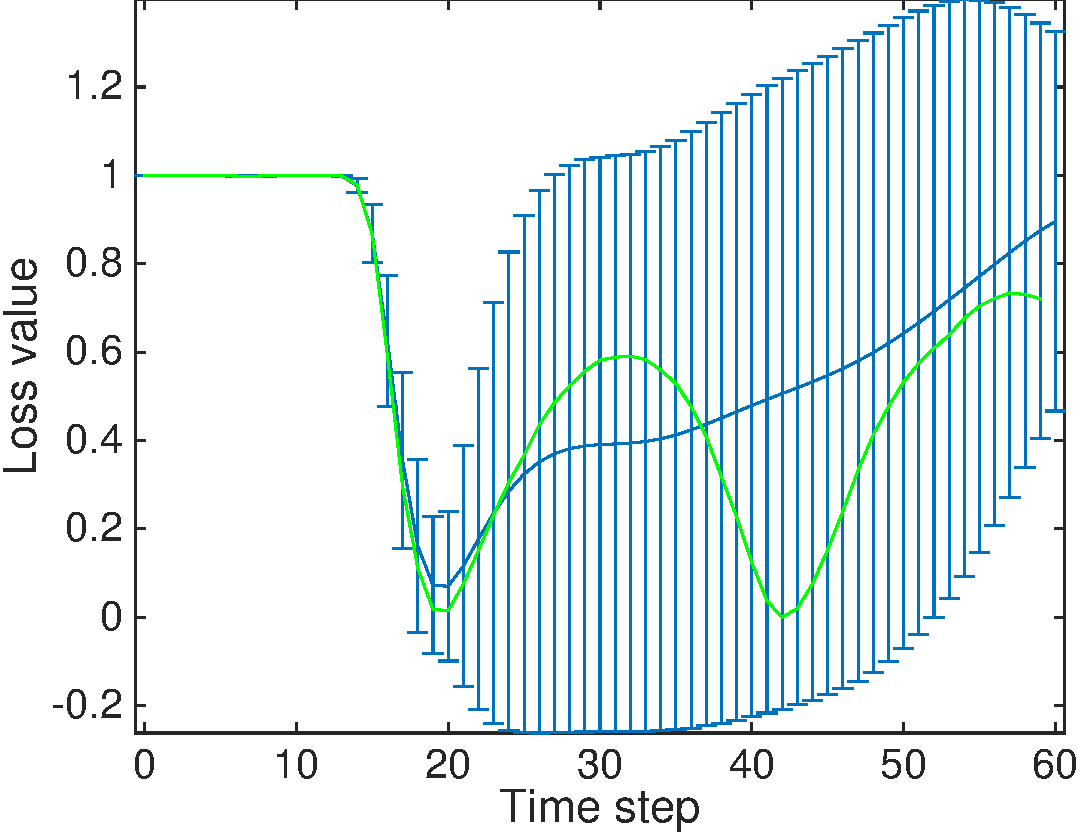
\includegraphics[width=60mm,scale=1]{plots/smk_loss}}{\caption{The predicted loss value of the trained controller for the single pendulum with the second order Markov representation. The green line corresponds to the rollout .}\label{fig:exps:single:2loss}}
    \ffigbox[\FBwidth][\FBheight][t]{\includegraphics[width=60mm,scale=1]{plots/smk_pred_x}}{\caption{The predicted trajectory of $x$. The blue error bars correpond to the variance multiplied by $2$.}\label{fig:exps:single:2predx}}
    \end{floatrow}
    \begin{floatrow}
    \ffigbox[\FBwidth][\FBheight][t]{\includegraphics[width=60mm,scale=1]{plots/smk_pred_theta}}{\caption{The predicted trajectory of $\theta$.}\label{fig:exps:single:2predtheta}}
    \ffigbox[\FBwidth][\FBheight][t]{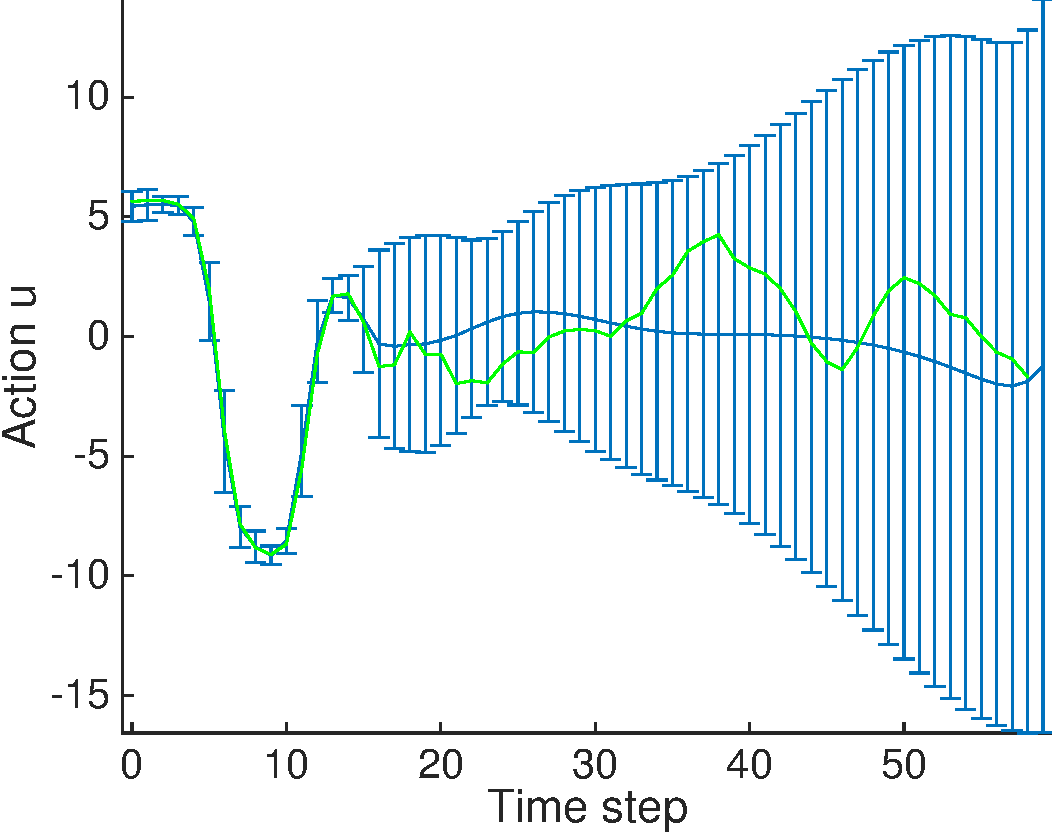
\includegraphics[width=60mm,scale=1]{plots/smk_pred_u}}{\caption{The predicted action applied to the pendulum.}\label{fig:exps:single:2predu}}
    \end{floatrow}
\end{figure}

\noindent The Figure \ref{fig:exps:single:2loss} shows the predicted loss value of the trained controller, where the Figures \ref{fig:exps:single:2predx}-\ref{fig:exps:single:2predu} show the predicted trajectory of $x$ and $\theta$ and the predicted action $u$ applied to the pendulum. First, the controller swings up the pendulum by applying positive action i.e. $5$ for few time steps, which is follow by maximum negative action i.e. $-10$. At that moment, the cart is heading towards its original position, but the pendulum is approaching the upright position\ (i.e. $\theta=0$). Then, the controller degrades its action to $0$, so the pendulum will actually slow down in the upright position and cart itself will stop around the origin.  Once this happens at $t=20$, the controller should start reacting depending on in which direction the pendulum wants to fall. At that time, the prediction on the state of the trajectory is not so tight anymore, since the controller is only reacting to the changes in the system. The prediction on trajectory matches the real rollout (i.e. green line), which means  the dynamics model is correct. More rollouts were made to determine the matching of the distribution to the samples.

\noindent Although the controller can keep the pendulum in the upright position, it does not guarantee to do it with the cart at the origin. To investigate it further, we linearize the policy at the target of the policy i.e. $ox=0, o\theta=0, x=0, \theta=0$: 
\begin{equation} \label{eq:exps:smk}
u=0.3007 + 0.07 \times (ox-0) + (-0.23) \times (\theta-0) \nonumber
\end{equation}
The weights of the $ox$ and $\theta$ seems small, which means that the controller is not so aggressive. This is likely to be because the variables are noisy. If the controller uses noisy variables to higher extent, it would inject further noise into the system making it more difficult to control. Tough, we have seen previously that the noise levels on the variables are relatively small according to our dynamics model. However, the noise could be also explained as the model uncertainty under the GP model. This would not be seen in the noise levels of our dynamics model.

\noindent Assuming that the dynamics model is correct, it seems that there are too much noise for the controller to do any better. As an experiment, the third order Markov representation is tried for modeling the dynamics. The bigger state representation should provide more information, which, possibly, should make the dynamics modeling easier. Indeed, the model with third Markov order representation yields better marginal likelihood for the same test dataset. Furthermore, the linear part of the GP models more complicated relationships between the variables:
\begin{equation}
\theta^{*} = 1.69 \times \theta - 0.43 \times o \theta -0.26 \times oo\theta + 1.07 \times x - 1.87 \times ox + 0.77 oox
\end{equation}
where $oo\theta$ and $oox$ stand for the angle and the cart position from the even older frame. New linear model for $\theta$ is interested not only in current angular velocity, but also in the previous one. Furthermore, $1.07 \times x - 1.87 \times ox + 0.77 oox$ is an acceleration filter on a cart position. For the same velocity of the cart $\dot{x}$, it will not have almost contribution  to the prediction of the next $\theta$. 

\noindent Another set of the experiments was run for the third order Markov representation. The new state of the system is:
\begin{equation}
[ooou, oox, oo\theta, oou, ox, o\theta, ou, x, \theta, u] \nonumber
\end{equation}
There were still two variables to predict i.e. $ou$ and $\theta$. The other settings of the experiments were the same as previously. During the training, there was no need to increase the amount of the pseudo points from $50$ to $100$. The successful controller was trained around iteration $14$, this kept training till the iteration $20$, so the total exposure time remains similar. 

\begin{figure}[!ht]
    \centering
    \begin{floatrow}
    \ffigbox[\FBwidth][\FBheight][t]{\includegraphics[width=60mm,scale=1]{plots/smk3_loss}}{\caption{The predicted loss value of the trained controller for the single pendulum with the thrid order Markov representation. The green line corresponds to the rollout .}\label{fig:exps:single:3loss}}
    \ffigbox[\FBwidth][\FBheight][t]{\includegraphics[width=60mm,scale=1]{plots/smk3_pred_x}}{\caption{The predicted trajectory of $x$.}\label{fig:exps:single:3predx}}
    \end{floatrow}
    \begin{floatrow}
    \ffigbox[\FBwidth][\FBheight][t]{\includegraphics[width=60mm,scale=1]{plots/smk3_pred_theta}}{\caption{The predicted trajectory of $\theta$.}\label{fig:exps:single:3predtheta}}
    \ffigbox[\FBwidth][\FBheight][t]{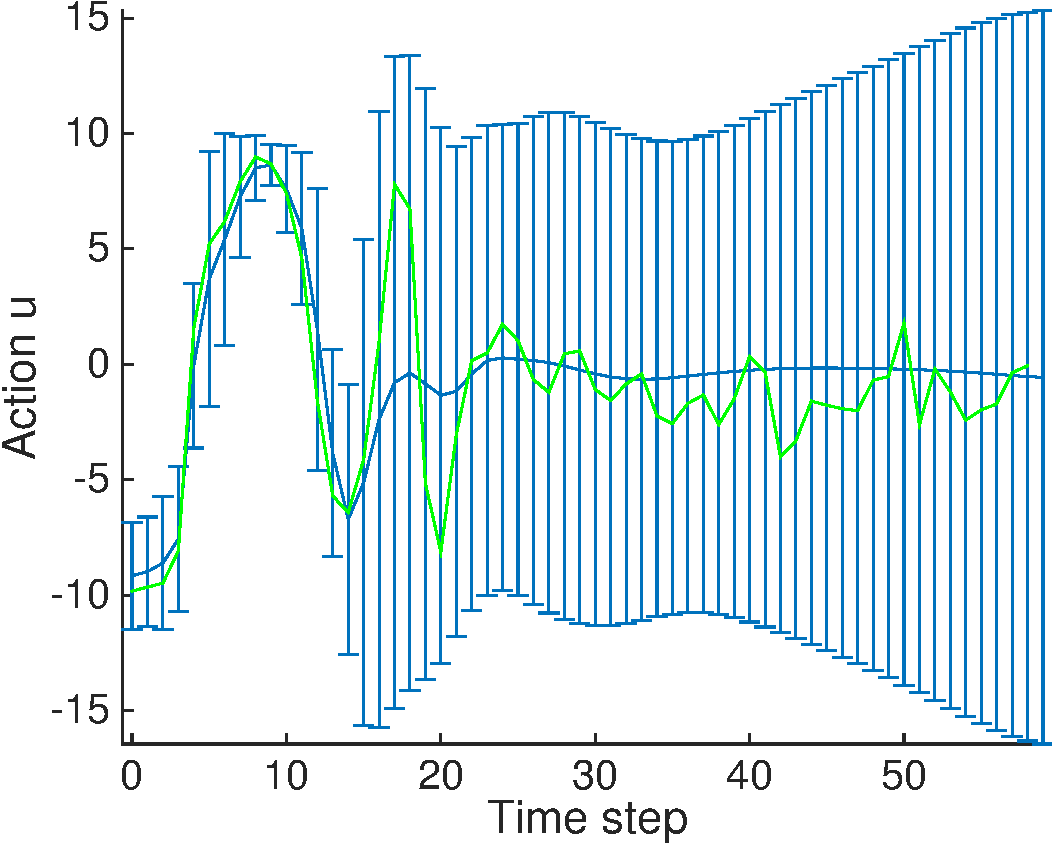
\includegraphics[width=60mm,scale=1]{plots/smk3_pred_u}}{\caption{The predicted action applied to the pendulum.}\label{fig:exps:single:3predu}}
    \end{floatrow}
\end{figure}

\noindent The Figure \ref{fig:exps:single:3loss} shows the predicted loss value of the new trained controller, where the Figures \ref{fig:exps:single:3predx}-\ref{fig:exps:single:3predu} show the predicted trajectory. In comparison to the trajectory shown on the Figures \ref{fig:exps:single:2predx}-\ref{fig:exps:single:2predu}, we can see that the state is better contained for later time steps i.e., lower error bar on the cart position and the angle. Similarly to the equation \ref{eq:exps:smk}, the controller is linearized at the upright position:
\begin{equation}
u=0.2831 + 1.08 \times (oox-0) + 1.08 \times (ox-0) + 1.08 \times (ox-0) + (-0.2) \times (\theta-0) \nonumber
\end{equation}
The new controller is more aggressive than the previous one. It assigns higher weights to the cart positions $oox, ox and x$. It also reacts depending on the current velocity of the cart, if there is any. Finally, it is also worth highlighting that the new controller swings the pendulum in other direction than the old one. This just experimentally shows that the original task is symmetric.

\subsection{Double pendulum}
\label{s:exps:double}
The experiments with the double pendulum were also run. In those experiments, the inner pendulum has a length of $12.5$ cm and the outer pendulum is longer, having the length of $22.7$ cm. We use the third order Markov representation for the state:
\begin{equation}
[ooou, oox, oo\theta_{1}, oo\theta_{2}, oou, ox, o\theta_{1}, o\theta_{2}, ou, x, \theta_{1}, \theta_{2}, u] \nonumber
\end{equation}
where $\theta_{1}$ represents the angle of the inner pendulum and $\theta_{2}$ of the outer one. The state has $12$ variables in total, where $3$ of those variables need to be predicted i.e. 3 separate GP models in our PILCO framework. Initially, $50$ pseudo points were used for the dynamics modeling. After the rollout nr $15$, the amount of the pseudo points was increased to $100$.

\noindent For the single pendulum, we specified the time horizon $T$ once and kept it the same through the whole task of learning. This does not seem enough to successfully learn the double inverted pendulum problem. The time horizon indirectly specifies what PILCO should learn. The Figure \ref{fig:exps:policytradeoff} compares the predicted loss of the two policies trained with different time horizon, but the same dynamics model. The blue error bars correspond to the policy with time horizon $T=40$, whereas the red blue bars represent the policy with $T=30$. The red policy performs better than the blue one with the exception of the last time step. The red controller swings up the pendulum faster, which allows it to achieve the upright position sooner and to have a tighter prediction on the state\ (time steps: 25-27). However, the upright state is lost immediately at time step 30, when the blue policy starts performing better. The blue policy trained on the longer time horizon prefers to swing up the pendulum slower, but then to have more chances to stabilize it in the upright position.

\begin{figure}[H]
\centering
\includegraphics[width=0.5\textwidth, scale=0.5]{plots/compare_pols}
\caption{\label{fig:exps:policytradeoff} The comparison of the predicted loss: the blue error bars represent the policy trained over the time horizon $T=40$, whereas the red error bars is the policy trained over $T=30$.}
\end{figure}

\noindent On the other hand, if the time horizon is too long, this has the implications for the dynamics model. There will be more samples for the dynamics model, but most of them will come from the regions of space, which are not crucial for successfully learning the whole task. In another series of the experiments, the time horizon was set to $60$. PILCO managed to learn how to swing up the first pendulum\ (time step $10-15$), but could not succeed on swinging up both pendulums\ (time step $15-25$). Then, instead of making further progress on it, PILCO started optimizing what actions to take when both pendulums are already dropped at time steps $40-50$. This may be also just an indicator that the dynamics model is not correct and the policy just adapts to this scenario. The longer rollouts also mean longer training time of the dynamics model. For our experiments with the double pendulum, we decided to start with time horizon $T=30$, and then, keep increasing it by another $5$ times steps if we think that we are dealing with the situation similar to the one from the previous paragraph.

\subsubsection{Sequence of linear models as policy representation}
\label{s:exps:double:policyrep}
The double inverted pendulum is more challenging problem, which requires more rollouts to learn the successful controller. After each rollout, the policy is being retrained from the previous optimal controller. One may be afraid whether the policy will not become too convoluted after many epochs of training. Indeed, it was noticed around the iteration nr $40$ that the policy learning did not continue to progress any more tough the dynamics model did. The mean cost of the predicted trajectory could be no further optimized. As mentioned earlier, the RBF network was used as a policy model. The Figure \ref{fig:exps:rbfactt} shows the mean output contributions of the individual units of the RBF network along the predicted trajectory. In optimization, some of those contributions need to change in order the controller to have the new predicted trajectory with lower mean cost. However, some of those contributions are not only high values, but they also cancel each other out. The Figure \ref{fig:exps:rbfcancel} shows how two high values contributions when added result in relatively small contribution function. Two units are highly coupled, the slight change in the position or height of one unit will result in significantly different function. This situation is not preferable for optimization, since it can not easily optimize any of those units. 

\begin{figure}[!ht]
    \centering
    \begin{floatrow}
    \ffigbox[\FBwidth][\FBheight][t]{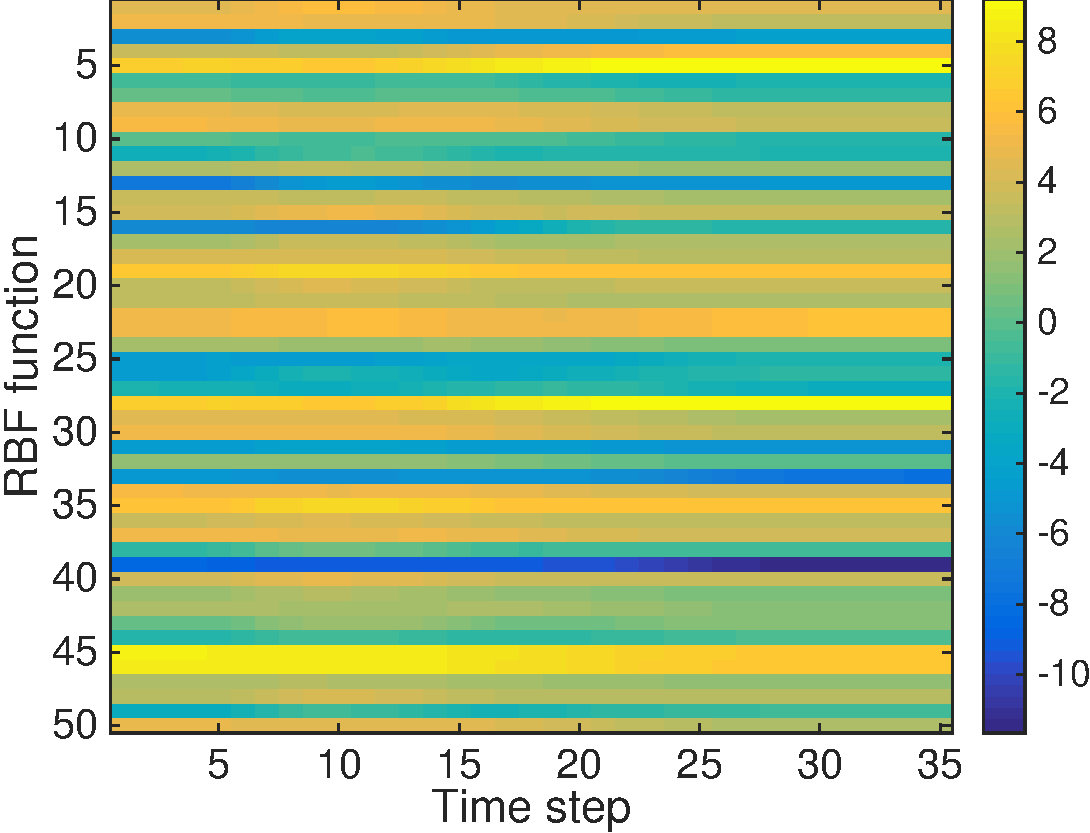
\includegraphics[width=60mm,scale=1]{plots/rbf_actt}}{\caption{The mean output contributions of the individual units of the RBF network along the predicted trajectory of the trained controller. The absolute values of those contributions are shown in the logarithm space (i.e. color value of $8$ corresponds to $29810$).}\label{fig:exps:rbfactt}}
    \ffigbox[\FBwidth][\FBheight][t]{\includegraphics[width=60mm,scale=1]{plots/rbf_cancel}}{\caption{The contribution for the predicted tracjectory of the unit $5$\ (blue line) and unit $28$\ (red line) of the RBF network. The contribution from both units cancel out when added\ (yellow line).}\label{fig:exps:rbfcancel}}
    \end{floatrow}
\end{figure}

\noindent To mitigate the above problem, the RBF policy has been converted to the sequence of linear models proposed in this dissertation \ref{s:pilco:seqlin}. The output distribution from the RBF policy is always approximated by moment matching. The linear output distribution is computed at each time step along the predicted trajectory to obtain the sequence of the linear models. This new policy will apply exactly the same actions as the RBF controller. However, the separate linear models do not infer over time, and thus, are unlikely to become highly coupled. This seems crucial for further successful learning that the controller can be optimized over many rollouts without getting convoluted.

\noindent Knowing that just one linear controller $\overline{\pi}$ can stabilize the double pendulum in the upright position, one may wonder how the sequence of the linear models will cope with the stabilization task itself. A successful sequence of linear models controller should simply duplicate $\overline{\pi}$ controller $T$ times. We believe that this will be indeed achieved in the training procedure. If the first controller $pi_{0}$ of the sequence is successfully learned and matches the $\overline{\pi}$ controller, then we can assume that the output state distribution after applying the action from that controller will be the same as the input distribution for that controller. That simply means that as a result of applying the new action, the state of the system did not change. With some simplification, we know that this should be true, since the controller aims to keep the pendulum in the upright position. If the one model of the sequence is successfully learned and the output state does not change, the next linear model of the sequence will be also learned since the same dynamics model is used. By induction, the whole sequence of the linear models will be successfully learned.

\subsubsection{Dynamics model}
\label{s:exps:double:dyns}
Around the rollout nr $50$, the sequence of the linear models arrived at the suboptimal parameters, which did not change over the next few rollouts. As we said in the previous section, the new policy model is very flexible to be optimized, since the separate linear models do not interfere over time. The policy training does not progress any further, since the dynamics model does not provide the policy with any new information. The dynamics model is either not good enough or there is simply too much noise in the system to successfully learn the task.  

\noindent The trained GP Time-Series model has $0.22^{\circ}$ process noise on the $theta_{1}$ prediction, which is propagated to the consecutive latent states of the time series model. It is not clear whether this process noise stops the policy from progressing. To address this issue, the experiment with learning only the subtask of the main task was proposed. The policy gives us the predicted trajectory of the state, which spans over the time horizon $T=40$. We can freeze our policy and dynamics model over first $20$ time steps and try to learn the new task from the time step $t=21$ onward. The separate dynamics model can be used only for this subtask. One can select the dynamics samples from each rollout just basing on time i.e. take the second half of each rollout\ (from $t=21$ onward). The dynamics model trained this way has the process noise on $theta_{1}$ close to $0$, instead the observation noise is close to  $0.22^{\circ}$. This is preferable behaviour of the model, since the observation noise is not going to be propagated through the time-series model. On the other hand, the dynamics model for the new subtask has a process noise of $0.13$ on $theta_{2}$. 

\noindent The policy was also trained for the new subtask using its new dynamics model. The policy performs better than the main policy from time step $t=21$ onward in the main task. The difference between two policies is even higher if the time boundary is chosen as $t=18$\ (the main policy has a tight prediction on the state at that time step). The Figure \ref{fig:exps:subtask:loss} compares the predicted loss of both controllers. The policy of the subtask has tighter predicition around the upright position\ (i.e. time steps $23-26$). On the Figure \ref{fig:exps:subtask:theta2}, we can also see how better the prediction on the $\theta_{2}$ angle is in the policy of the subtask in comparison to the old policy. With the new subtask controller, $20$ rollouts were conducted, which confirmed that the prediction on the trajectory matches the samples from the real system.

\begin{figure}[!ht]
    \centering
    \begin{floatrow}
    \ffigbox[\FBwidth][\FBheight][t]{\includegraphics[width=60mm,scale=1]{plots/compare_subtask_loss}}{\caption{The comparison of loss of the predicted trajectory from time step $t=18$. Blue error bars correspond to the main policy, while the green are the subtask's policy.}\label{fig:exps:subtask:loss}}
    \ffigbox[\FBwidth][\FBheight][t]{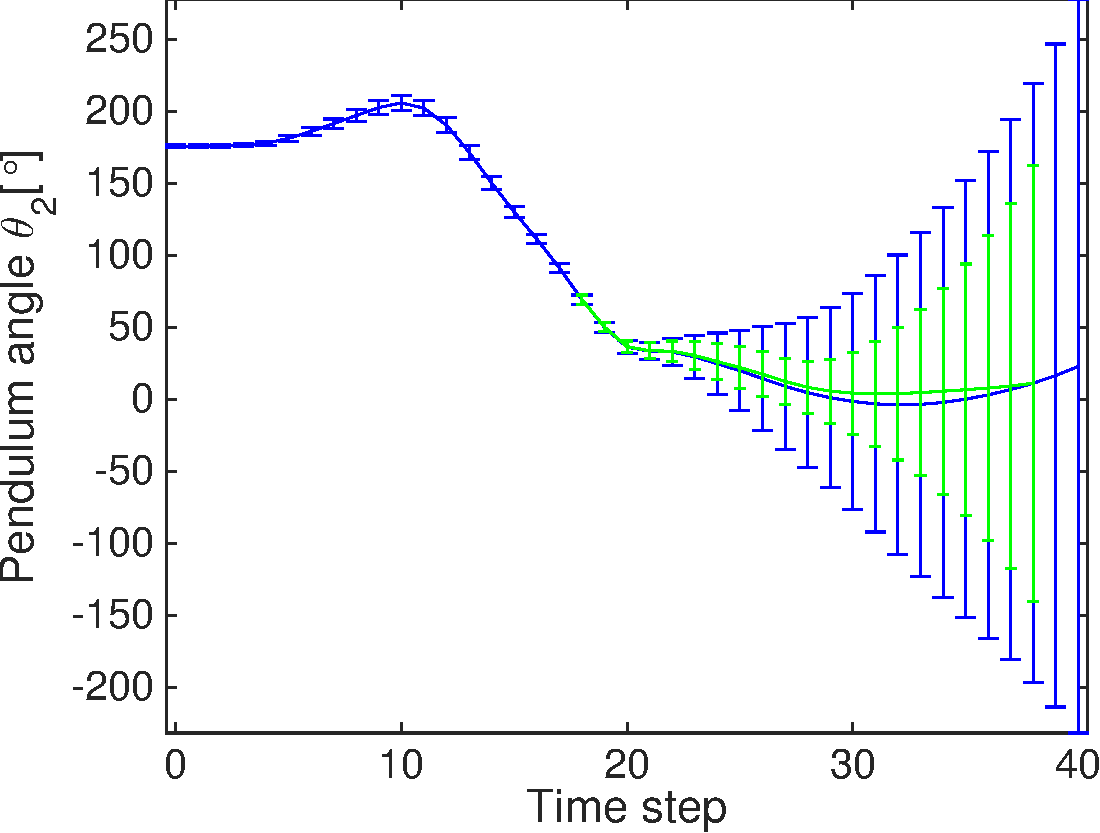
\includegraphics[width=60mm,scale=1]{plots/compare_subtask_theta2}}{\caption{The comparison of the predicted trajectory according to the main policy\ (blue) and subtask's one\ (green).}\label{fig:exps:subtask:theta2}}
    \end{floatrow}
\end{figure}

\noindent The results of the above experiment indicate that the previously trained dynamics model is not good enough. It is possible that one parametric GP model is not able to capture the whole dynamics of the system. The GP is used with squared exponential which is a stationary covariance function. The dynamics of the double pendulum may be non-stationary. The pendulum behaves differently when it is being swung up with high angular velocity and when it slows down around the upright position. This dynamical system can be also tackled by using more GPs in the time-series model as it is proposed in this dissertation\ (section \ref{s:pilco:ssm}). Effectively, the task can be split onto smaller subtasks, which can be learned in joint optimization.

\noindent If more GPs are plugged to the time-series model, the samples may be assigned to different GPs also  on state-based criterion. Instead of splitting the samples by time, we can filter the rollout which pass through the specific state distributions. For example, if we want to model the subtask of stabilizing the pendulum, we can filter only those parts of rollouts in which latent state or observation itself is in upright position. The dynamics models with such a state filtering have been also trained. Such a compound dynamics model yields slight improvement into the policy. Another extension to the Direct Method for GP Time-series model proposed in this dissertation\ (section \ref{s:pilco:ssm}) is training pseudo inputs. Although the method has worse time complexity, it was used to determine whether the time-series model with one GP would perform better. It turns out that the trained model with the movable pseudo inputs overfits the data by yielding unrealistic low noise levels. 

\noindent When modeling high dimensional problem, the FITC algorithm may tend to put the pseudo points on the sphere of the data points, instead of putting them next to the training points. This results in the higher variance in the regions of the training points. The marginal likelihood optimization should try to the pseudo points next to the training points, but this may not happen. This phenomenon could be a possible reason of the problems we encounter while using the GP tim-series dynamics model. In the time-series model, the locations of the pseudo points are pre-trained by FITC. The non time-series GP model, which does not account for the noise in the input was also trained on the whole accumulated data. This was followed by training new policy model, which seems promising. In simulations, the controller thinks that it can successfully control the double inverted pendulum. However, the samples from the real system do not match the predicted trajectories.

\subsubsection{Controller}
\label{s:exps:double:ctrl}
The predicted loss and the trajectory of the best trained controller are shown on the Figures \ref{fig:exps:double:3loss}-\ref{fig:exps:double:3predu}. The controller uses three separate dynamics model which are split by time: the first GP for time steps from $1$ to $18$, the second GP from $19$ to $25$ and the last GP from $26$ to $40$. All of the dynamics model are trained in joint optimization, as well as the main policy consisting of policies of the three subtasks.  The total exposure time was $112$ seconds, which corresponds to $3386$ training samples.

\noindent The controller first swings up the outer pendulum in the similar fashion to the controller in the single pendulum problem: by applying few times strong positive action followed by the series of strong negative actions. The swing up of the outer pendulum happens just before time step $t=20$. Then, the outer pendulum is pushed out, which is followed by the swinging up of the inner pendulum. As the result of the swinging up two pendulums, the pendulum are close to being  colinear. At time step $t=27$, the angle of the first pendulum first pendulum is $-10^{\circ}$, where the angle of the second pendulum is $10^{\circ}$. The mean predictions on those angles go steadily in opposite direction, which means that the pendulums are expected to become colinear. However, the prediction on the time step $t=30$ is not tight enough for the pendulums to be guaranteed to become colinear. Nevertheless, then, the pendulums tried to be stabilize. It happened once on twenty additional rollouts that the pendulums were actually stabailized till the end of the time horizon\ (this would not be a case if the time horizon was longer). Under the simulations, we have also observed that the algorithm tries to swing up both of the pendulums at the beginning at the same time. This is achieved by slowly swinging the pendulum in both directions. However, as a result, the pendulums are already colinear when they approach the upright position.

\begin{figure}[!ht]
    \centering
    \begin{floatrow}
    \ffigbox[\FBwidth][\FBheight][t]{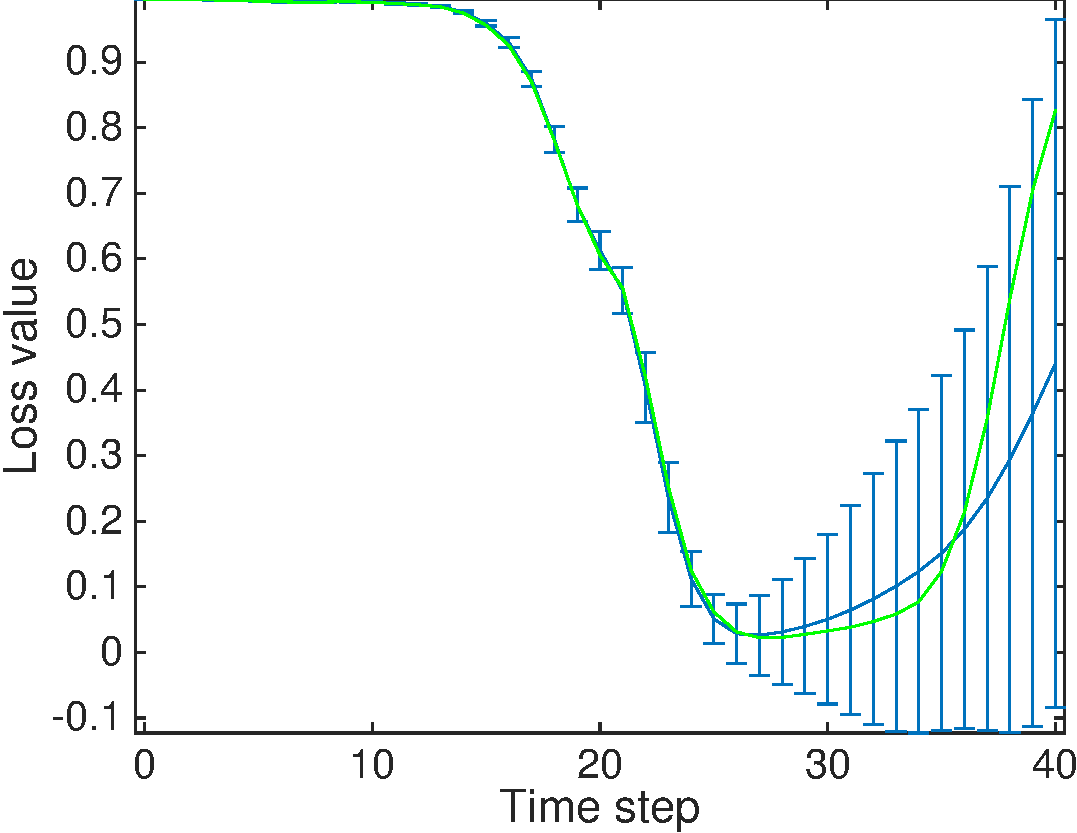
\includegraphics[width=60mm,scale=1]{plots/dmk3_loss}}{\caption{The predicted loss value of the trained controller for the double pendulum with the thrid order Markov representation. The green line corresponds to the rollout .}\label{fig:exps:double:3loss}}
    \ffigbox[\FBwidth][\FBheight][t]{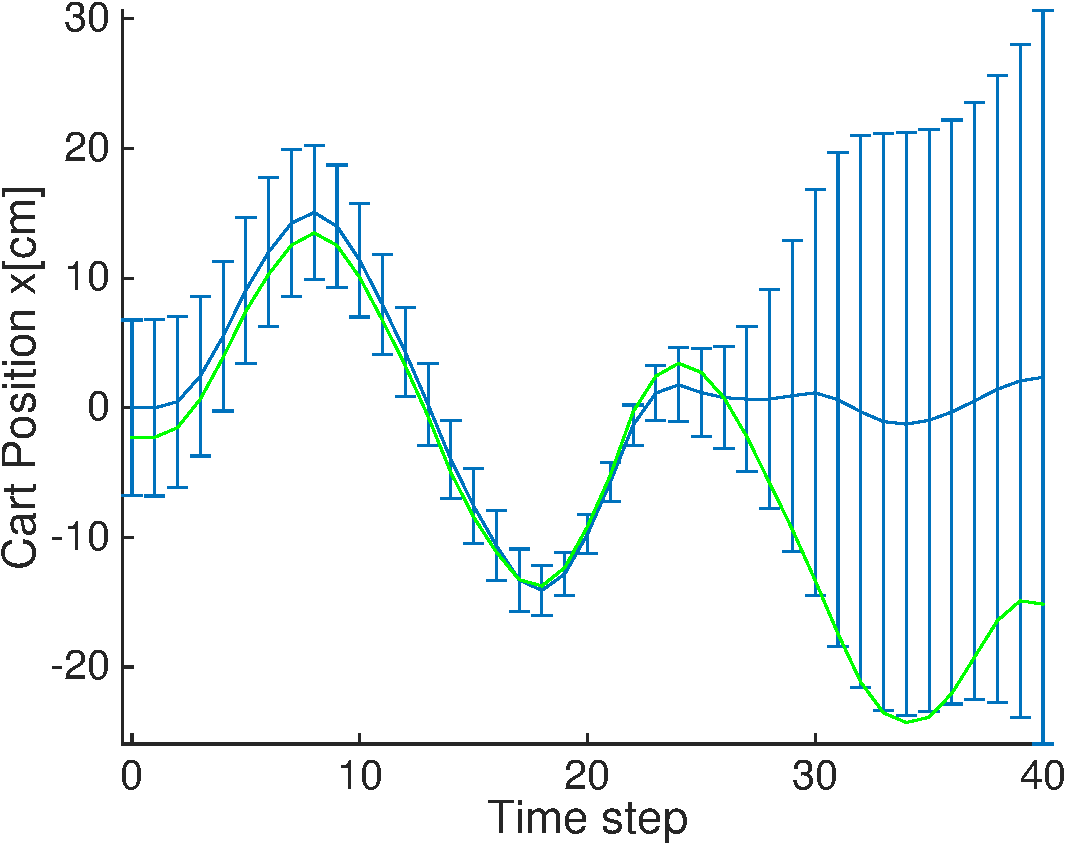
\includegraphics[width=60mm,scale=1]{plots/dmk3_pred_x}}{\caption{The predicted trajectory of $x$.}\label{fig:exps:double:3predx}}
    \end{floatrow}
    \begin{floatrow}
    \ffigbox[\FBwidth][\FBheight][t]{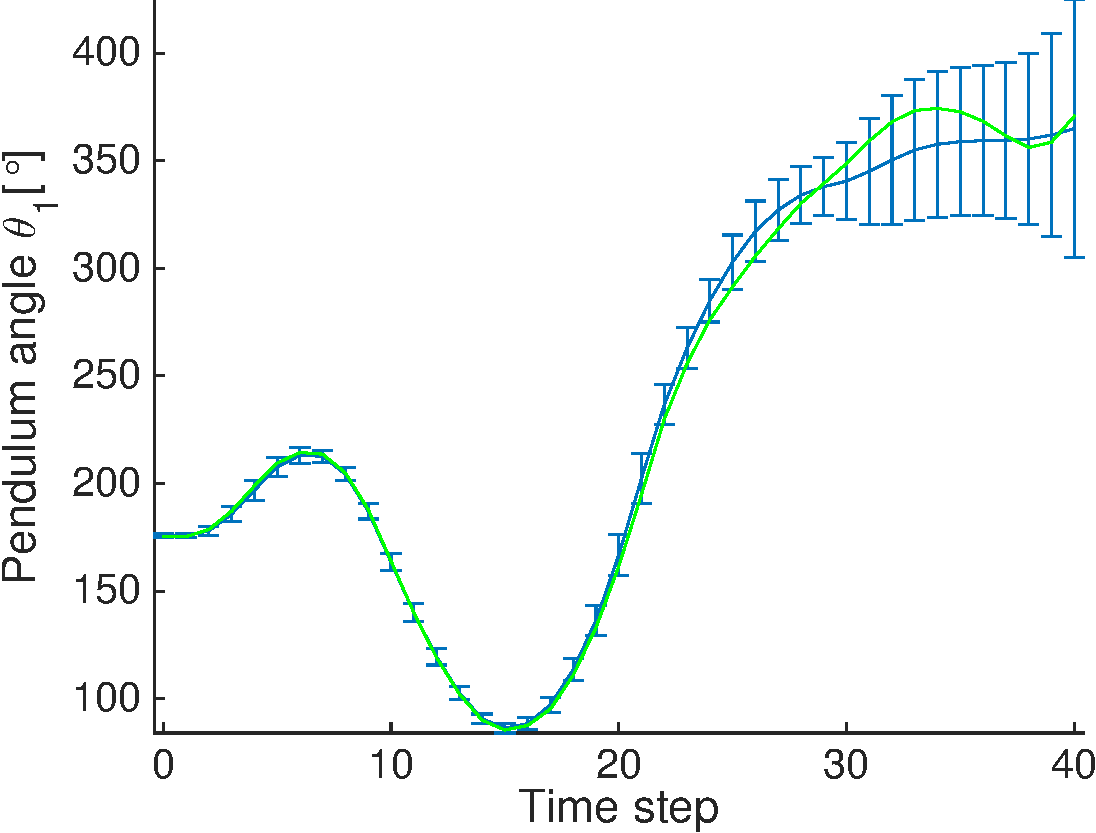
\includegraphics[width=60mm,scale=1]{plots/dmk3_pred_theta1}}{\caption{The predicted trajectory of $\theta_{1}$.}\label{fig:exps:double:3predtheta1}}
    \ffigbox[\FBwidth][\FBheight][t]{\includegraphics[width=60mm,scale=1]{plots/dmk3_pred_theta2}}{\caption{The predicted trajectory of $\theta_{2}$.}\label{fig:exps:double:3predtheta2}}
    \end{floatrow}
    \begin{floatrow}
    \ffigbox[\FBwidth][\FBheight][t]{\includegraphics[width=60mm,scale=1]{plots/dmk3_pred_u}}{\caption{The predicted action applied to the pendulum.}\label{fig:exps:double:3predu}}
    \end{floatrow}
\end{figure}
\section{Conclusions}
\label{s:con}
The PILCO framework was applied the 

 


In the project, PILCO is applied to the real 


-managed to make single pendulum work - third order representation
-investigate issues related to double pendulum.
this resulted in the improvement of the PILCO framework: the sequence of the linear models,
not convoluted
investigated that the direct method for GP time-series model is not good enough dynamics model for the problem
-extend it by having more than one parametric model
-although manage to swing it up and there are trials to keep it balanced, the task remains unsuccesful. 


\bibliographystyle{abbrvDOI}
\bibliography{dissertation}

\appendix
\end{document}
